% \documentclass[10pt,a4paper,twoside, twocolumn]{article}

\documentclass[%
 aip,
% aps,
% jmp,
% bmf,
% sd,
% rsi,
% jap,
cha,
 amsmath,amssymb,
%preprint,%
 reprint,%
%author-year,%
%author-numerical,%
% Conference Proceedings
]{revtex4-1}

% PREAMBLE
%%IDIOMAS:
\usepackage[spanish,english]{babel} %Poner es-tabla para que ponga los caption en español. El último idioma que se cargue es el que se queda por defecto. Luego en el texto se puede cambiar con \selectlanguage{idioma}.
\usepackage[utf8]{inputenc}	%Para los acentos

%PARA ESCRIBIR EN COLOR:
\usepackage{color}	%Para escribir en color con el comando \textcolor{color}{texto}
\usepackage[dvipsnames]{xcolor} %Paquete con colores predefinidos extra

%PARA USAR TIPOGRAFÍA DE CONJUNTOS
\usepackage{amssymb}

%PARA CAMBIAR EL TIPO DE FUENTE (LETRA):
%Por defecto tenemos Computer Modern (no es necesario cargar ningun paquete), pero podemos seleccionar otro tipo de letra.
%Cargamos un paquete para cada tipo de letra:
%\usepackage{times} %fontcode ptm
%\usepackage{palatino} %fontcode ppl
%\usepackage{bookman} %fontcode pbk
%\usepackage{helvet} %fontcode phv
\usepackage{courier} %fontcode pcr
%Tras cargar el paquete, podemos cambiar la letra haciendo: {\fontfamily{fontcode}\selectfont  texto}

%PARA DIVIDIR EL TEXTO EN COLUMNAS:
\usepackage{multicol}		%Para dividir el texto en columnas con \begin{multicols}{nº de columnas\end{multicols}
\setlength{\columnsep}{0.5cm} %Para elegir la separación entre las columnas.

%INDENTADO Y MÁRGENES:
%Para el indentado (sangría de los párrafos).
\usepackage{indentfirst}	%Para que indente el primer párrafo tras un título de sección.
\setlength{\parindent}{0.5cm}	%Tamaño de la sangría.
%Para eliminar la sangría de un párrafo hacemos: {\setlength{\parindent}{0pt} texto del párrafo}

%Para los márgenes:
\usepackage{anysize}	
%\marginsize{3cm}{3cm}{1.5cm}{1.5cm}	%Indicamos los márgenes {izquierda}{derecha}{arriba}{abajo}
%\usepackage[top=0cm, bottom=1.5cm, inner=2cm, outer=2cm, headheight=3cm, includeheadfoot]{geometry} %Indicamos los márgenes para encuadernación.
\usepackage[top=1.5cm, bottom=3cm, inner=2cm, outer=2cm]{geometry} %Indicamos los márgenes para encuadernación.


%GRÁFICOS (PAQUETES PARA INTRODUCIR IMÁGENES):
%\usepackage[pdftex]{graphicx}
\usepackage{graphicx}
\DeclareGraphicsExtensions{.png,.jpg,.pdf,.mps,.gif,.bmp,.eps}
\usepackage{glossaries}
\usepackage{tikz}
\let\ig\includegraphics 

%Uso de flotantes en imágenes y tablas:
\usepackage{float}
\usepackage{subfig}

%Para modificar los captions de imágenes y tablas:
\usepackage[margin=0cm,font=footnotesize]{caption} 

%Para el uso de psfrag:
\usepackage{psfrag}
\usepackage{pstool}
\usepackage{epsfig}
\usepackage{graphics}

%Para incluir figuras mezcladas (en paralelo) con el texto:
\usepackage{wrapfig}

%Paquetes para tikz
\usepackage{pgf,tikz}
\usepackage{mathrsfs}
% \usetikzlibrary{arrows}
% \usetikzlibrary{angles,calc,intersections,quotes,arrows.meta}
% \usetikzlibrary{arrows.new}
\newcommand{\degre}{\ensuremath{^\circ}}

%ENCABEZADOS Y PIES DE PÁGINA:
\usepackage{fancyhdr}
%\pagestyle{fancyplain}
%\headheight=60pt %para cambiar el tamaño del encabezado
%\lhead{\includegraphics[width=0.08\textwidth]{MARCA_UMA.png}}
%\chead{ANTEPROYECTO \\}
%\rhead{\includegraphics[width=0.2\textwidth]{logo_etsii.jpg}}
%\renewcommand{\headrulewidth}{1.5pt} % grosor de la línea de la cabecera
%\renewcommand{\footrulewidth}{1.5pt} % grosor de la línea del pie de página

%Explicación:
%\comando[pagina par]{pagina impar}
%Nota: para incluir una imagen en el encabezado o pie de página, en caso de incluirla dentro de los corchetes [], es necesario meter el comando \includegraphics[opciones]{figura} entre corchetes {}.

%Encabezados:
\pagestyle{fancyplain}
%\lhead[\thepage]{Documento de tipo {\em article}}
%\chead[]{}
%\rhead[Manual básico de \LaTeX]{\thepage}
%\renewcommand{\headrulewidth}{0pt}

%Ejemplo encabezado con figuras:
\pagestyle{fancyplain}
\lhead[]{}
\chead[]{}
\rhead[]{}
\renewcommand{\headrulewidth}{0pt}
%\lhead[{\includegraphics[width=0.1\textwidth]{logo_uc3m.eps}}]{\includegraphics[width=0.1\textwidth]{logo_uc3m.eps}}
%\chead[]{}
%\rhead[{\includegraphics[width=0.3\textwidth]{logo_nanotec.eps}}]{\includegraphics[width=0.3\textwidth]{logo_nanotec.eps}}
%\renewcommand{\headrulewidth}{1pt}

%Pie de pagina:
\lfoot[\thepage]{}
\cfoot[]{}
\rfoot[]{\thepage}
\renewcommand{\footrulewidth}{0pt}

%Primera pagina de un capitulo (solo book):
\fancypagestyle{plain}{
\fancyhead[L]{}
\fancyhead[C]{}
\fancyhead[R]{}
\fancyfoot[L]{}
\fancyfoot[C]{}
\fancyfoot[R]{}
\renewcommand{\headrulewidth}{0pt}
\renewcommand{\footrulewidth}{0pt}
}
\pagestyle{fancy}

%NUMERACIÓN DE LAS SECCIONES Y SU INCLUSIÓN EN EL ÍNDICE:
\setcounter{secnumdepth}{6} %Para que numere las subsubsecciones y los paragraph
\setcounter{tocdepth}{6} %Para que introduzca las subsubsecciones y los paragraph en el índice
% Do not indent paragraphs nor subparagraphs
\makeatletter
\renewcommand\paragraph{\@startsection{paragraph}{4}{\z@}%
                                      {-3.25ex\@plus -1ex \@minus -.2ex}%
                                      {0.0001pt \@plus .2ex}%
                                      {\normalfont\normalsize\bfseries}}
\renewcommand\subparagraph{\@startsection{subparagraph}{5}{\z@}%
                                      {-3.25ex\@plus -1ex \@minus -.2ex}%
                                      {0.0001pt \@plus .2ex}%
                                      {\normalfont\normalsize\bfseries}}
\makeatother

%Esto es para que numere las tablas, ecuaciones y figuras según el capítulo en el que estén (solo para tipo book).
%\numberwithin{table}{chapter}
%\numberwithin{equation}{chapter}
%\numberwithin{figure}{chapter}

%ENUMERACIONES:
\usepackage{enumerate}

%TABLAS:
\usepackage{booktabs}	% Para aumentar grosor de tablas.
\usepackage{multirow}	% Para poder unir filas y columnas en las tablas.
\usepackage{colortbl}	% Para colorear tablas.
%\usepackage{slashbox}	% Para colocar una línea diagonal dividiendo las celdas.
\usepackage{makecell}
\usepackage{array}
\usepackage{pdflscape}  % Para incluir páginas apaisadas compilando con pdflatex
\usepackage{lscape}     % Para incluir páginas apaisadas compilando con latex

%Para lineas más gruesas en tablas:
%\thickhline >> línea horizontal de espesor definido en height
%' >> para columna interior, línea vertical de espesor definido en width (en lugar de |c|, ponemos 'c') 
%! >> para primera columna a la izquierda, línea vertical de espesor definido en width (en lugar de |c|c|..., ponemos !c|c|...)
%? >> para primera columna a la izquierda, línea vertical de espesor definido en width (en lugar de ...|c|c|, ponemos ...|c|c?)
\makeatletter
\newcommand{\thickhline}{%
    \noalign {\ifnum 0=`}\fi \hrule height 2pt
    \futurelet \reserved@a \@xhline
}
\newcolumntype{'}{@{\hskip\tabcolsep\vrule width 2pt\hskip\tabcolsep}}
\newcolumntype{!}{@{\vrule width 2pt\hskip\tabcolsep}}
\newcolumntype{?}{@{\hskip\tabcolsep\vrule width 2pt}}
\makeatother

%Para columnas de ancho fija:
\newcolumntype{L}[1]{>{\raggedright\let\newline\\\arraybackslash\hspace{0pt}}m{#1}}
\newcolumntype{C}[1]{>{\centering\let\newline\\\arraybackslash\hspace{0pt}}m{#1}}
\newcolumntype{R}[1]{>{\raggedleft\let\newline\\\arraybackslash\hspace{0pt}}m{#1}}

%Para unir columnas:
%\multicolumn{nº de columnas}{alineación}{texto}
%Para unir filas:
%\multirow{nº de filas}{ancho}[desplazamiento vertical]{texto}
%Para colorear filas:
%\rowcolor[rgb]{0,1,1}Roque & Fort \\
%\rowcolor[cmyk]{0.5,0,0,0.1}Abraham & Lapuerta \\
%Para colorear columnas (se emplea al definir las columnas o con el multicolumn):
%\begin{tabular}{|>{\columncolor[rgb]{0.7,0,0.7}} c |
%Para definir un color:
%\definecolor{micolor}{rgb}{0,1,0.5}
%Para escalar la tabla al ancho de página:
%\resizebox{<ancho_deseado>}{!} {<entorno tabular que se desea escalar>}

%MATEMÁTICAS Y SÍMBOLOS:
%Para introducir formulas matemáticas alinedas (align y align*):
\usepackage{amsmath,bm}
%\usepackage{amsmath,amssymb,amsfonts,latexsym}

%Símbolo del euro:
\usepackage{eurosym} %Para escribir el símbolo del euro se emplea \euro.

%HIPERVÍNCULOS:
% \usepackage[linktocpage]{hyperref}
\usepackage[linktocpage,breaklinks=true]{hyperref}
\hypersetup{
colorlinks = true,
%linkcolor  = Red,
%citecolor  = Red,
linkcolor  = MidnightBlue,
citecolor  = OliveGreen,
urlcolor   = blue
}

%CREAR COMANDOS PROPIOS
%Creamos un comando (\courier) para cambiar la letra:
\newcommand*{\courier}{\fontencoding{\encodingdefault}\fontfamily{pcr}\fontseries{m}\fontshape{n}\selectfont}
\newcommand*{\couriernegrita}{\fontencoding{\encodingdefault}\fontfamily{pcr}\fontseries{b}\fontshape{n}\selectfont}
%Creamos un comando para poner el símbolo de marca registrada:
\newcommand*{\R}{$^{\textregistered}$}
%Creamos el comando parcial de primer orden:
\providecommand{\parcial}[2]{\frac{\partial #1}{ \partial #2}}
%Creamos el comando parcial de segundo orden:
\providecommand{\pparcial}[2]{\frac{\partial^2 #1}{ \partial #2 ^2}}

%PARA INTRODUCIR CÓDIGO DE MATLAB, FORTRAN:
\usepackage{listings}
%\usepackage[]{mcode}	% Paquete de formato especial para MATLAB.
%\lstinputlisting{nombre_del_documento.m}
\definecolor{mygreen}{RGB}{28,172,0} % color values Red, Green, Blue
\definecolor{mylilas}{RGB}{170,55,241}
\definecolor{mybrown}{RGB}{165,42,42}

% Para poner los captions de los códigos en español:
\renewcommand{\lstlistingname}{Código}
% Para poner los captions de los códigos en inglés:
%\renewcommand{\lstlistingname}{Code}
% Para poner el índice de códigos en español:
% Documento en español:
\renewcommand\lstlistlistingname{Índice de códigos}
% Documento en inglés:
%\renewcommand\lstlistlistingname{List of Codes}

%Para introducir código Matlab:
\lstdefinestyle{MATLAB}{
	language=Matlab,%
    %basicstyle=\color{red},
    breaklines=true,%
    morekeywords={matlab2tikz},
    keywordstyle=\color{black},%
    morekeywords=[2]{1},
    keywordstyle=[2]{\color{mylilas}},
    identifierstyle=\color{black},%
    stringstyle=\color{mylilas},
    commentstyle=\color{mygreen},%
    showstringspaces=false,%without this there will be a symbol in the places where there is a space
    numbers=left,%
    numberstyle={\tiny \color{black}},% size of the numbers
    numbersep=9pt, % this defines how far the numbers are from the text
    emph=[1]{for,end,break,if,elseif,else,switch,case,otherwise,while,function,global},emphstyle=[1]\color{blue}, %some words to emphasise  
    emph=[2]{all,on}, emphstyle=[2]\color{mylilas},
}

% Para introducir código Fortran:
\lstdefinestyle{FORTRAN}{
	language=[90]Fortran,
    %basicstyle=\color{red},
    breaklines=true,%
    morekeywords={matlab2tikz},
    keywordstyle=\color{mybrown},%
    morekeywords=[2]{1}, 
    keywordstyle=[2]{\color{mybrown}},
    identifierstyle=\color{black},%
    stringstyle=\color{mylilas},
    commentstyle=\color{blue},%
    showstringspaces=false,%without this there will be a symbol in the places where there is a space
    numbers=left,%
    numberstyle={\tiny \color{black}},% size of the numbers
    numbersep=9pt, % this defines how far the numbers are from the text
    emph=[1]{real,pointer},emphstyle=[1]\color{mygreen}, %some words to emphasise  
    emph=[2]{type}, emphstyle=[2]\color{mybrown},
}

%PARA INTRODUCIR ARCHIVOS PDF EN EL DOCUMENTO:
\usepackage[final]{pdfpages}
%\includepdf[pages=inicial-final]{nombre_del_documento}\usepackage[pdftex]{graphicx}
%NOTA: Es necesario compilar con pdfLaTeX, por lo que hay que cargar este paquete para que las imágenes en .eps no den problemas.
\usepackage{epstopdf}

%PARA INTRODUCIR TEXTO DE RELLENO:
\usepackage{lipsum}
%\lipsup[numero de parrafo inicial - numero de parrafo final]

%PARA VARIAS CITAS BIBLIOGRAFICAS SEPARADAS POR GUION
\usepackage{cite}
%HASTA AQUÍ EL PREÁMBULO DEL DOCUMENTO. AHORA COMIENZA EL DOCUMENTO EN SÍ.
%%%%%%%%%%%%%%%%%%%%%%%%%%%%%%%%%%%%%%%%%%%%%%%%%%%%%%%%%%%%%%%%%%%%%%%%%%%%%%%%%%%%%%%%%%%%%%%%%%%%%%%%%%
%%%%%%%%%%%%%%%%%%%%%%%%%%%%%%%%%%%%%%%%%%%%%%%%%%%%%%%%%%%%%%%%%%%%%%%%%%%%%%%%%%%%%%%%%%%%%%%%%%%%%%%%%%

%\usepackage{mathabx} % For \widebar command 
\usepackage[normalem]{ulem}
\usepackage{moresize}
\usepackage[export]{adjustbox}


\usepackage{comment}
\usepackage[dvipsnames]{xcolor} 
\usepackage{graphicx}
\usepackage{bm}

\usepackage[linktocpage,breaklinks=true]{hyperref}
\hypersetup{
colorlinks = true,
%linkcolor  = Red,
%citecolor  = Red,
linkcolor  = MidnightBlue,
citecolor  = OliveGreen,
urlcolor   = blue
}


\newcommand{\ad}[1]{{\color{red} #1}}
\newcommand{\jz}[1]{{\color{blue}\textbf{JZ: #1}}}
\providecommand{\ea}[1]{\textcolor{magenta}{#1}}

\renewcommand{\thefootnote}{$*$}



% DOCUMENT 
\begin{document}

% TITLE AND ABSTRACT NO revtex4-1 -----------------------------------
\title{Modelling of a Hall thruster plume: influence of plume boundary conditions and size, and cathode location}


% Force line breaks with \\
\author{A. Domínguez-Vázquez}
\email{adoming@uma.es}
\affiliation{Universidad de Málaga, 29071 Campanillas, Spain}
%Lines break automatically or can be forced with \\
 
\author{J. Zhou}
\affiliation{Universidad Carlos III de Madrid, 28911 Leganés, Spain}
\author{A. Sevillano-González}
\affiliation{Universidad Carlos III de Madrid, 28911 Leganés, Spain}
\author{E. Ahedo}
\affiliation{Universidad Carlos III de Madrid, 28911 Leganés, Spain}

\date{\today}% It is always \today, today,
             %  but any date may be explicitly specified



\begin{abstract}
    The current-free plasma plume of a Hall effect thruster is investigated through a 2D axisymmetric hybrid (particle-in-cell/fluid) model and code. First, since the simulated plume is necessarily finite, attention is paid to the boundary conditions at the plume boundary P. A novel global plume condition (GPC) model, which directly imposes the global current-free condition at P and determines the potential far downstream, is implemented. This is compared with the widely used local plume condition (LPC) model, which over-forces the current-free condition by imposing zero current density locally at P, thus artificially distorting plasma plume characteristics. Second, the influence of the cathode location on plume characteristics, electron current paths, and the cathode-to-plume coupling voltage is studied in detail. Configurations with centrally and laterally-mounted cathodes are compared. Central cathodes have better discharge performance due to the improved cathode-beam coupling. Laterally-mounted cathodes behave very differently depending on whether they are located inside or outside a magnetic separatrix (MS) surface, generally present in the plume. MS-external cathodes present much worse cathode-plume coupling. These trends with the cathode location are in line with previous experimental and numerical studies. Finally, the influence of the plume size has been assessed within all the above studies: the GPC, with a much better physical basis than the LPC, makes the plume solution less dependent on plume size; and the MS-external lateral cathodes are more affected by plume sizes and thus require working with larger plume domains.
\end{abstract}

\maketitle


%%%%%%%%%%%%%%%%%%%%%
\section{Introduction}\label{sec: intro}
%%%%%%%%%%%%%%%%%%%%%


In the near plume of a Hall effect thruster (HET) complex physical processes take place that remain not fully understood, and which play an important role in thruster performances and its integration with other spacecraft systems.
Specifically, the neutralization of the expanding plasma jet and the interaction between the ion beam and the electron flow emitted from the neutralizer cathode are influenced by several factors, including the cathode's position \cite{till99,jame07,beal07,hofe08b,mcdo09,somm08}, its relative placement within the magnetic configuration \cite{somm11b,tura16,yu17,ding18}, and the electrical setup of the testing facilities \cite{frie14,frie16a,walk16a,walk16b}.
Consequently, progress towards the development of an accurate and predictive model for the near plume of a HET is of significant importance.

Many hybrid models, implementing a particle-in-cell (PIC) formulation for heavy species (ions and neutrals) and a fluid model for electrons \cite{fife98,hage02,parr06a,garr06,somm07,pera22b,cich21a}, and multi-fluid \cite{mike12b,keid04,ande18b} models used in HET research typically simulate the plasma discharge inside the thruster channel and in a limited plume region.
Simulating large plumes is computationally expensive and plume truncation is unavoidable. However, for a precise characterization of the discharge performance, simulations must include a sufficiently large portion of the plume.  Effects of plume truncation on the numerical solution and, in particular, uncertainties on the boundary conditions (BCs) to be applied at the outflow boundary, can hinder the validation of simulation models against experimental data from plasma diagnostics in the near plume. 
Therefore, setting appropriate BCs at the downstream plume boundary of the finite simulation domain is of central importance.
In particular, these must be consistent with the current-free character of the plasma beam in the far plume and the decay of the electric potential towards a uniform downstream value, representing either the infinity of free space or the metallic walls of a large vacuum chamber.


The most widely adopted approach to BCs is a local plume condition (LPC) model, which sets the plasma current to zero locally, i.e., at any point along the plume boundary \cite{mike12b,parr06a,pera22b}.
Clearly, this is an overforced way of satisfying  the global current-free condition. Furthermore, zero local electric current (also known as current ambipolarity) is not satisfied at the  internal points of the plasma beam. Thus, the LPC is going to artificially distort the plasma beam properties.
%
For instance, Ref. \citenum{orte16} noted that H6 thruster multi-fluid simulations with LPC required to place the downstream boundary at a distance of at least 10 channel lengths downstream the thruster exit plane to avoid artificially increased electron transport across magnetic lines due to the zero local current condition.
%
Moreover, as we will show below, the LPC model is somewhat arbitrary in providing conditions for the electron temperature or its gradient at the boundary and does not determine the final electric potential in the plume. For instance, Ref. \citenum{mike09} finds that the temperature solution in the near field (from about three channel lengths downstream the thruster exit) is largely driven by the prescribed boundary value, which is informed from plasma measurements.
Therefore, to be consistent, this approach requires accurate electron temperature measurements in the plume, which may be only available for a limited range of operational conditions.

The first main goal of the paper is to present an alternative global plume condition (GPC) model, which enforces directly the global current-free condition at the plume boundary, determining simultaneously the electric potential at infinity required for that. Finally, the knowledge of this potential allows for determining the electron energy flux at the plume boundary.

The relative location of the external hollow cathode (in charge of emitting the necessary electron flows to current-neutralize the emitted ion beam and to ionize the neutral gas) is known to be important in the characteristics of the plasma plume. We need to distinguish first between laterally and centrally-mounted cathodes.
In the near plume of HET with a conventional (i.e., non-shielded) magnetic topology, a null magnetic point at the axis typically exists, wherefrom a magnetic separatrix (MS) surface develops towards the external walls of the thruster, separating closed and open magnetic field lines. 
Several experimental studies have shown a significant impact on performance and plasma variables if a laterally-mounted cathode is positioned either inside or outside the MS \cite{somm11b,tura16,yu17,ding18}. In the last case, a higher cathode coupling voltage is expected to bring part of the electron emission into the thruster channel.
A centrally-mounted cathode emits along the axis, which is a second magnetic separatrix. Experimental \cite{jame07,hofe08b} and numerical \cite{cho17,cao20} studies 
comparing laterally and centrally mounted cathodes have reported lower plume divergence and higher efficiency when the cathode is located at the thruster axis. 
The second main goal of the paper is to analyze the above three cathode locations and show the influence on the plasma plume characteristics.

The third, complementary goal is to analyze the influence of the size of the external numerical domain on the plasma plume
for the different BCs and cathode locations.  
For that purpose, four different plume sizes will be considered.
As commented above, very large domains are difficult to deal with because of the highly irregular MFAM (and have a high computational cost, of course). Very short domains do not allow enough plasma expansion, and the solution is more affected by the selected BCs, which are always an approximation of the effect of the non-simulated far plume. The influence of the BCs on the plasma plume are expected to be more acute with the restrictive LPC than with the GPC, and for lateral cathodes located externally to the MS.


All analyses in this paper will be based on numerical simulations of a 5kW-class HET, 
conducted using the axisymmetric hybrid PIC/fluid code HYPHEN \cite{domi19a,domi19b,pera22b}.
The rest of the paper is organized as follows. Sec. \ref{sec: HYPHEN_code} presents the GPC model and its implementation within HYPHEN. Sec. \ref{sec: comp_local_GDML} compares the simulation results obtained with both the GPC and LPC models for four plume sizes, with the laterally-mounted cathode placed inside the MS. Sec. \ref{sec: cathode location} presents the results for both the GPC and LPC models and for a laterally-mounted cathode outside the MS and a centrally-mounted cathode. Finally, Sec. \ref{sec: conclusions} summarizes the conclusions.




%%%%%%%%%%%%%%%%%%%%%%%%%%%%%%%%%%%%%%%%%%%%%%%%%%%%%%%%%%%
\begin{figure}[!t]
\centering
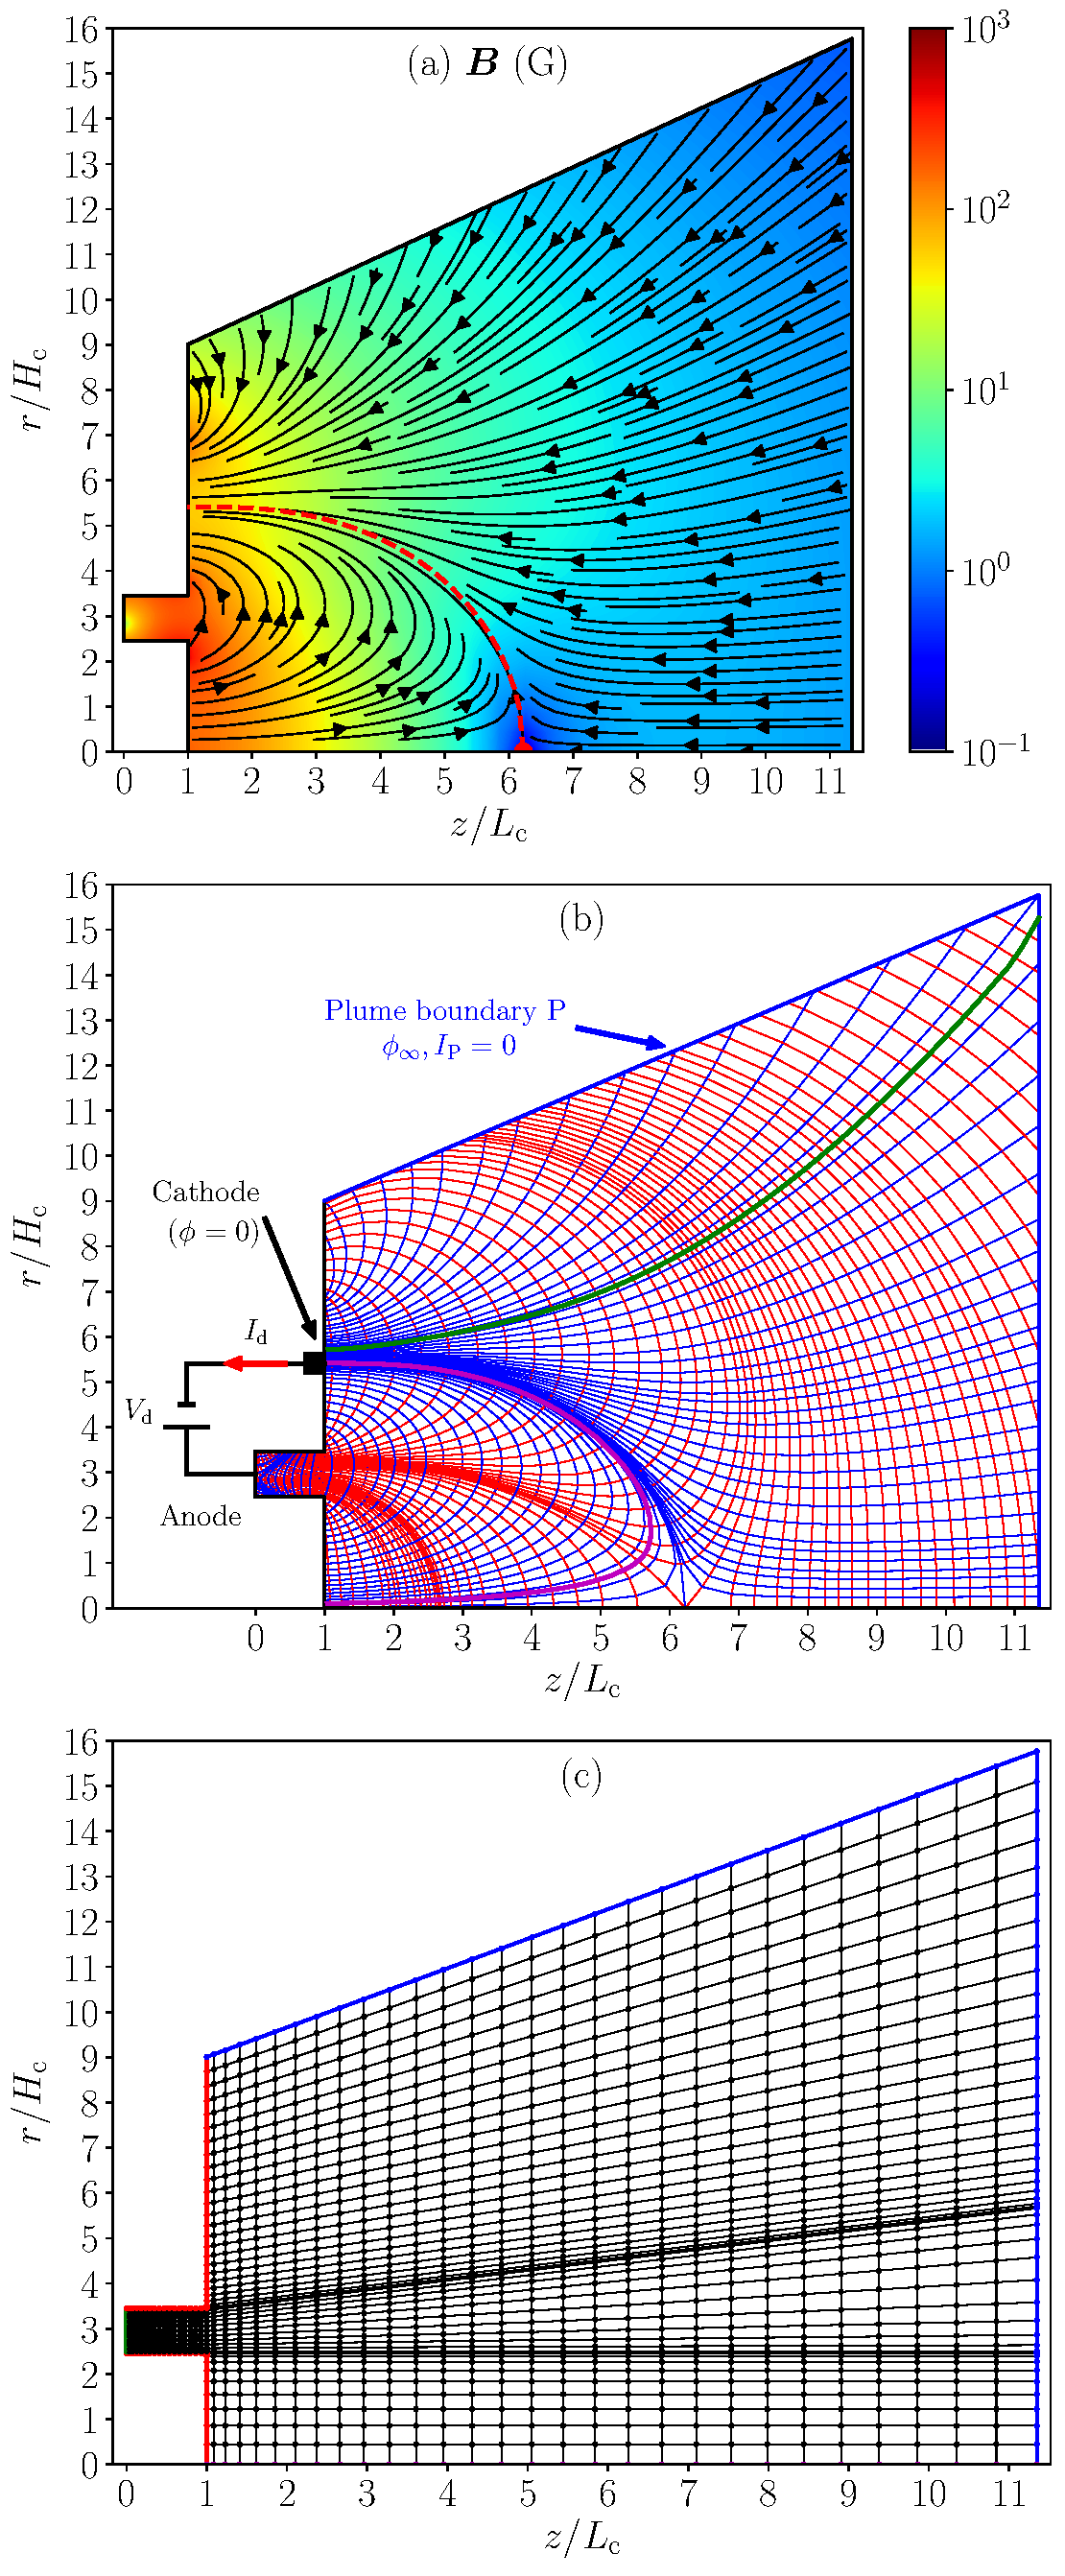
\includegraphics[width=0.85\columnwidth]{figures/fig1.pdf}
\caption{(a) 2D ($z$,$r$) contour map and streamlines of $\bm B$. The dashed red line corresponds to the MS, and the red circle marker indicates the magnetic singular point. (b) The MFAM used by the E-module. Inner blue and red lines are $B$-parallel and $B$-perpendicular lines, respectively, defining the cells. The magenta and green lines correspond to the CML for cathodes 1 and 2, respectively. (c) The PIC mesh used by the I-module. The red, green and magenta lines indicate the thruster dielectric walls, the anode wall and the symmetry axis, respectively. All figures correspond to plume size P3.
} 
\label{fig: domain_meshes}
\end{figure}
%%%%%%%%%%%%%%%%%%%%%%%%%%%%%%%%%%%%%%%%%%%%%%%%%%%%%%%%%%%

    
%%%%%%%%%%%%%%%%%%%%%
\section{Simulation details}\label{sec: HYPHEN_code}
%%%%%%%%%%%%%%%%%%%%%


\subsection{Setup and model}
A 5 kW-class HET similar to a PPS5000 \cite{duch19,duch23}, with a conventional (non-shielded) magnetic topology and a hollow cathode is considered for this study. Figs. \ref{fig: domain_meshes}(a)-(c) sketch the simulation domain, which comprises the thruster annular vessel (with length $L_\mathrm{c} = 29$ mm, width $H_\mathrm{c} = $ 22.2 mm, and inner radius 54.5 mm), and a near-plume region of different sizes. Fig. \ref{fig: domain_meshes}(a) shows the applied magnetic field $\bm B$ magnitude map and streamlines. The peak of $B \equiv |\bm B|$ along the thruster channel midline is 196.05 G, at $z/L_\mathrm{c} = 0.86$. The dashed red line in Fig. \ref{fig: domain_meshes}(a) indicates the (off-axis) MS in the near plume, which passes through the magnetic singular point located at the axis at $z/L_\mathrm{c} = 6.2$. The magnetic lines are represented by the blue lines in Fig. \ref{fig: domain_meshes}(b).  
%
Downstream of the MS, the magnetic topology exhibits a magnetic nozzle (MN) shape, which will channel the plasma beam in the far plume \cite{ahed10f}.
%


The thruster anode covers the complete channel back wall and the cathode, located at the thruster exit plane, can be either laterally-mounted (i.e., off-axis), as depicted in Fig. \ref{fig: domain_meshes}(b), or centrally-mounted (i.e., at the axis).
%
A power source sets a discharge voltage $V_\mathrm{d} = 300$ V between anode and cathode. The reference of the electric potential $\phi$ is set at the cathode, so that the potential of the anode wall is $V_\mathrm{d}$. 
%
The thruster operates with xenon and the total neutral mass flow rate injected into the domain is $\dot{m} = \dot{m}_\mathrm{A} + \dot{m}_\mathrm{C}$, where $\dot{m}_\mathrm{A} = 17.59$ mg/s and $\dot{m}_\mathrm{C} = 1.32$ mg/s are the flow rates injected through the anode and the cathode, respectively (details on neutral injection conditions can be found in Ref. \citenum{pera22b}).
%
The discharge current $I_\mathrm{d}$ collected at the anode wall provides the electron flow injected at the cathode. The temperature of the electrons emitted from the cathode is set to 2.25 eV.

The plasma discharge is simulated with the axisymmetric hybrid code HYPHEN, whose characteristics have been detailed in previous works \cite{domi19a,zhou21,zhou22a,pera22b} and are briefly outlined next.
%
The code is composed of three main modules coupled within a time-marching sequential loop. The ion (I)-module operates on a structured mesh of the simulation domain, shown in Fig. \ref{fig: domain_meshes}(c), and implements a PIC method to solve the dynamics of the heavy species (i.e., ions and neutrals, including singly and doubly charged ions; charge exchange collisions (CEX) generating slow ions and fast neutrals in the plume are also considered) obtaining the net ion density $n_\mathrm{i}$ and ion current density vector $\bm j_\mathrm{i}$.
%

The electron (E)-module solves a quasineutral drift-diffusion fluid model for the magnetized electron population on an unstructured magnetic field align mesh (MFAM) \cite{pere16}, obtained from $\bm B$ and shown in Fig. \ref{fig: domain_meshes}(b), where red lines correspond to magnetic equipotential lines.
%
Setting the plasma density $n_\mathrm{e}=n_\mathrm{i}$, it provides the solution for the electric potential $\phi$, the electron temperature $T_\mathrm{e}$, the electron current density vector $\bm{j}_\mathrm{e}$ (and thus the electric current density vector $\bm j = \bm j_\mathrm{e} + \bm j_\mathrm{i}$), and the energy flux vector $\bm{P}''_\mathrm{e} = 5n_\mathrm{e}T_\mathrm{e}\bm{u}_\mathrm{e}/2 + \bm{q}_\mathrm{e}$ (sum of enthalpy and heat fluxes). Full details on the electron fluid model equations can be found in Sec. III.A of Ref. \citenum{pera22b} and Sec. 2.1 of Ref. \citenum{zhou22a}; the numerical treatment of these equations is described in the Appendix B of Ref. \citenum{zhou22a}. Interpolation between the PIC mesh and the MFAM is required to transfer plasma properties.
%
The axisymmetric electron fluid model needs to be completed with empirical submodels for electron-wall interaction properties and for turbulent cross-field transport due to high-frequency plasma waves driven by kinetic and fluid instabilities. As in Ref. \citenum{pera22b}, the local electron turbulence level is modeled with a ``turbulent collisional frequency'' of the form  $\alpha_\mathrm{t}\omega_\mathrm{ce}$, with $\omega_\mathrm{ce} = eB/m_\mathrm{e}$ the electron cyclotron frequency and $\alpha_\mathrm{t}$ a ``step-out'' type tuning function with two parameters, $\alpha_\mathrm{t1}$ and $\alpha_\mathrm{t2}$,  empirically adjusted.
%
Each magnetic line is assigned a constant value of $\alpha_\mathrm{t}$, equal to either $\alpha_\mathrm{t1}$ or $\alpha_\mathrm{t2}$. The transition from $\alpha_\mathrm{t1}$ to $\alpha_\mathrm{t2}$ is set at the magnetic line that intersects the point $z/L_\mathrm{c} = 1.49$ at the channel midradius (located downstream of the $B$ peak along the channel midline).
%
The values $\alpha_\mathrm{t1} = 1.2\%$ and $\alpha_\mathrm{t2} = 4.8\%$ were found  adequate to fit the experimental values of $I_\mathrm{d}$ and thrust ($F$) of the PPS5000 at the operating point under consideration. 
%
Previous works have demonstrated the significance of accounting for the electron anomalous transport in the near plume on the cathode-beam coupling process \cite{orte16}. In this study, the values of $\alpha_\mathrm{t1}$ and $\alpha_\mathrm{t2}$ are kept the same for all simulation cases, regardless of plume size, BCs applied at the plume boundary and cathode locations.


Non-neutral effects are limited to (infinitely) thin Debye sheaths that develop around the thruster walls. The sheath (S)-module of HYPHEN solves these sheaths and provides BCs at the sheath edge for the electron fluid model. The Appendix of Ref. \citenum{pera22b} details the kinetic sheath model, which assumes the sheath to be planar, unmagnetized, collisionless, and electron-repelling. The model admits secondary electron emission,
net electric current, and an
electron velocity distribution function (VDF) with only a partial replenishment (here, a 30\%) of the tail of wall collected electrons. The model determines the local sheath potential fall from the quasineutral plasma to the wall at both the dielectric walls and the conducting anode. 
The implementation is described in Sec. III.A of Ref. \citenum{pera22b}.



%%%%%%%%%%%%%%%%%%%%%
\subsection{Simulation cases}\label{sec: sim_settings}
%%%%%%%%%%%%%%%%%%%%%   

Four different plume domains (P1 to P4) are considered, featuring plume axial extensions of 100, 200, 300 and 400 mm ($3.4L_\mathrm{c}$, $6.9L_\mathrm{c}$, $10.3L_\mathrm{c}$ and $13.8L_\mathrm{c}$). For all cases, the plume domain extends radially up to 200 mm at the thruster exit plane (see Fig. \ref{fig: domain_meshes}). The radial extension of the downstream end increases with the plume length and is set to 250, 300, 350 and 400 mm for P1 to P4 cases, respectively, so that the PIC mesh adapts to the ion beam expansion in the plume to limit particle depletion. As an example, Figs. \ref{fig: domain_meshes}(b) and (c) show the MFAM and the PIC mesh for domain P3, respectively. The main characteristics of the simulation domain meshes for plume sizes P1 to P4 are listed in Tab. \ref{tab: HET_sim_par}. 
The MFAM cell layout is optimized \textit{ad hoc} for each plume size. This may yield small mesh-related variations on plasma properties for different plume domains, as we comment later.


Each heavy species population (i.e., singly and doubly charged ions and neutrals) is controlled during the simulation by maintaining a target number of 200 and 500 macroparticles per cell (with a $\pm 10\%$ of tolerance) for plume sizes P1 and P2–P4, respectively.
%
The ion-moving timestep is set to 15 ns, ensuring that the fastest doubly charged ions require at least two timesteps to cross the smallest PIC mesh cell.
A total time of 900 $\mu$s is simulated, enough to capture a sufficiently large number of breathing mode cycles. All the numerical results in this work are averaged over several of these cycles.
%
Simulations are performed on a modern workstation using 30 threads 
and their computational time ranges from approximately 8 to 40 hours for plume sizes P1 to P4.



As outlined in Sec. \ref{sec: intro}, three distinct cathode configurations are considered: cathode 1 (C1) and cathode 2 (C2) correspond to an laterally-mounted cathode positioned inside and outside the MS at radial distances of 120 mm and 126.6 mm, respectively, while cathode 3 (C3) represents a centrally-mounted cathode aligned with the thruster axis. 
The magnetic field line passing through the center of the cathode injection surface will be referred to as the cathode magnetic line (CML), and it guides the trajectory of the central portion of the emitted magnetized electron beam.
The magenta and green lines in Fig. \ref{fig: domain_meshes}(b) represent the corresponding closed and open CML for C1 and C2, with the latter intersecting the downstream axial boundary below the top right corner of the plume domain. For C3 the CML coincides with the symmetry axis.
%
For plume size P1 and cathode C1, the axial downstream boundary of the plume intersects the closed CML and the magnetic singular point is left outside the plume domain. 
%
Hereafter, simulation cases for plume sizes P1 to P4 and cathode configurations C1 to C3 will be referred to as GP$i$C$j$ and LP$i$C$j$ ($i = 1, 2, 3, 4$; $j=1,2, 3$) for the GPC and LPC, respectively.




%%%%%%%%%%%%%%%%%%%%%%%%%%%%%%%%%%%%%%%%%%%%%%%%%%%%%%%%%%%
\begin{table}[!t]
\centering
\resizebox{1.0\columnwidth}{!}{
{\renewcommand{\arraystretch}{1.2}
\begin{tabular}{|l|c|c|}
\hline
Simulation parameter         & Units          & Value                  \\ \hline\hline
PIC mesh number of cells     & -              & 969, 1284, 1509, 1734  \\ \hline
PIC mesh number of nodes     & -              & 1049, 1371, 1601, 2831 \\ \hline
PIC mesh smallest grid size  & mm             & 1                      \\ \hline
MFAM number of cells         & -              & 1948, 2397, 3506, 4081 \\ \hline
MFAM number of faces         & -              & 4025, 4933, 7186, 8353 \\ \hline
MFAM average cells skewness  & (10$^{-2})$ -  & 7.06, 6.45, 5.49, 5.31 \\ \hline
\end{tabular}
}
}
\caption{Main mesh parameters (values separated by commas correspond to plume sizes P1 to P4).}
\label{tab: HET_sim_par}
\end{table} 
%%%%%%%%%%%%%%%%%%%%%%%%%%%%%%%%%%%%%%%%%%%%%%%%%%%%%%%%%%%



%%%%%%%%%%%%%%%%%%%%%
\subsection{Conditions at the plume boundary}\label{sec: GDML}
%%%%%%%%%%%%%%%%%%%%%

We consider the usual case where a current-free plasma beam from the thruster expands into free space (or into a large vacuum chamber with low background pressure). The blue line in Fig. \ref{fig: domain_meshes}(b) represents the boundary P of the simulated plume. BCs must be defined at each point on P, ensuring they are ``compatible'' with the expected plasma behavior between P and infinity.  For instance, the electric potential is expected to decrease monotonically to a value $\phi_\infty$ at infinity (relative to the cathode)  to comply with the current-free condition. This implies that ions exiting the simulated plume domain will ultimately reach infinity, while individual electrons leaving P may either reach infinity or be reflected back into the simulation domain. The electron fluid model requires BCs at P on the normal electron current  $j_\mathrm{neP} = \bm 1_\mathrm{n} \cdot \bm j_\mathrm{eP}$ (with $\bm 1_\mathrm{n}$ being the {\it outward} unit normal vector locally at P) and either the energy flux $P''_\mathrm{neP} =  \bm 1_\mathrm{n} \cdot \bm{P}''_\mathrm{eP}$ or the temperature $T_\mathrm{eP}$.

%
The conventional LPC model imposes zero local current, that is
%
\begin{equation}
j_\mathrm{neP} = -j_\mathrm{niP},
\label{eq: jneP local}
\end{equation}
%}
This is very simple to implement but, as discussed in Sec. \ref{sec: intro}, is a very forced way to comply with the global current-free condition. Furthermore, the LPC has not a way to determine the potential $\phi_\infty$ to sustain a zero current.


In the LPC model, the electron energy flux is set to
\begin{equation}
    P''_\mathrm{neP} = -cT_\mathrm{eP}j_\mathrm{neP}/e,
    \label{eq: PneP local}
\end{equation}
but there is no clear criterion for defining the  constant $c$.
2D hybrid HET simulations by Lam et al. \cite{lam15} applied a Neumann BC on $T_\mathrm{e}$, i.e.  $dT_\mathrm{e}/d\bm{1}_\mathrm{n} = 0$ (which is equivalent to $q_\mathrm{neP} = 0$) thus yielding $c = 5/2$.
HYPHEN simulations of an electrodeless plasma thruster\cite{zhou22a}, using $c =$ 5/2, 9/2, and 13/2, revealed a significant impact of $c$ on the electron temperature, with $c = 9/2$ providing the best agreement for two plume domain sizes.
HYPHEN simulations for a magnetically shielded HET\cite{pera22b} used $c = 9/2$, and this value will be used here with the LPC model.
Let us notice that other multi-fluid \cite{mike09,mike12b} and hybrid \cite{kubo17,parr06a} HET simulations with an LPC model have set (somehow arbitrarily) $T_\mathrm{eP}$, instead of $P''_\mathrm{neP}$, and multi-fluid simulations of a MN \cite{mark20a} found that $T_\mathrm{e}$ profiles are highly sensitive to the type of BC (i.e., Dirichlet, Neumann or Robin) is applied on $T_\mathrm{eP}$.



As a better physically-based alternative to the LPC, we propose here a global plume condition (GPC) which imposes directly the global zero current condition at P as
%
\begin{equation}
    I_\mathrm{P} = I_\mathrm{eP} + I_\mathrm{iP} = \int_\mathrm{P} [j_\mathrm{ne}(\phi_\mathrm{\infty P}) + j_\mathrm{ni}] dS = 0,
    \label{eq: GDML_zero_I}
\end{equation}
%
where: the surface integral is performed over P; $I_\mathrm{eP}$ and $I_\mathrm{iP}$ are the outwards electron and ion currents at P, respectively; $j_\mathrm{niP}$ is provided by the I-module at any point of P; and, assuming a quasi-Maxwellian VDF for electrons, $j_\mathrm{neP}(\phi_\mathrm{\infty P})$ comes out from 
%
\begin{equation}
j_\mathrm{neP}(\phi_\mathrm{\infty P}) = - en_\mathrm{eP}\sqrt{\frac{T_\mathrm{eP}}{2\pi m_\mathrm{e}}}
\exp \left(\frac{-e\phi_\mathrm{\infty P}}{T_\mathrm{eP}}\right), 
\label{eq: jne sheath}
\end{equation}
%
with $\phi_\mathrm{\infty P}=\phi_\mathrm{P}-\phi_\infty \geq 0$,
being $\phi_\mathrm{P}$ the local electric potential at the (quasineutral) plume boundary P.
%
Eq. \eqref{eq: GDML_zero_I} is an implicit equation for $\phi_\infty$, which is solved iteratively [by linearizing Eq. (\ref{eq: jne sheath})]. Thus, the resulting value of $\phi_\infty$ satisfies $I_\mathrm{P} = 0$. Once $\phi_\infty$ is known, $j_\mathrm{neP}$ at any point of P is given by Eq. \eqref{eq: jne sheath}. 
%
The GPC model can be readily extended to configurations where $I_\mathrm{P} \neq 0$, for instance, if the far field represents a vacuum chamber that is electrically connected to the cathode. Such generalization is not possible under the LPC, which constrains the solution by enforcing zero current density locally at every point of P.


Invoking again a quasi-Maxwellian electron VDF in the far plume, the electron energy flux at infinity would be $P''_\mathrm{ne\infty} = -2T_\mathrm{eP}j_\mathrm{neP}/e$.
Then, in the GPC model, the BC for the energy flux at P, dependent on $\phi_\infty$, is 
\begin{equation}
    P''_\mathrm{neP} = P''_\mathrm{ne\infty} -j_\mathrm{neP}\phi_{\infty P}=
    -j_\mathrm{neP}\frac{T_\mathrm{eP}}{e}\left(2+\dfrac{e\phi_{\infty P}}{T_{eP}}\right).
    \label{eq: energy_flux_P}
\end{equation}
Notice that the sum between parentheses would correspond here to the arbitrary constant $c$ in the LPC Eq. \eqref{eq: PneP local}.





%%%%%%%%%%%%%%%%%%%%%
\section{Influence of the boundary condition model and plume size}\label{sec: comp_local_GDML}
%%%%%%%%%%%%%%%%%%%%%  


Solutions for plume sizes P1 to P4 with C1, and using the GPC and LPC models, are compared here. We begin with the maps of electric and electron currents, as these are the most significantly affected. This is followed by the maps of scalar plasma variables, and finally, the performance results.



Fig. \ref{fig: j_comp_P1P4} plots the in-plane electric current density $\tilde{\bm\jmath}= \bm j - j_\mathrm{\theta}\bm 1_\theta$ for plume sizes P1 to P3 (P4 results are similar for GPC and LPC and thus omitted). All of them satisfy $I_\mathrm{P}=0$, [i.e. $I_\mathrm{iP} = |I_\mathrm{eP}|$ in all cases, according to Eq. \eqref{eq: GDML_zero_I}]. The BC at P affects mainly the $\bm{\tilde \jmath}$ solution downstream of the CML. In this region, the LPC forces artificially all current loops to close within the plume domain. Therefore, current loops outward of the CML are clearly different for different plume sizes. In contrast, with the GPC, current loops change less with the plume size since they are not constrained to close within the plume domain (the electric current at P can be locally nonzero), which, aside from being more consistent, makes the GPC more robust against plume truncation.
%

The LPC provides a good approximation only when the simulated plume domain is sufficiently large. In both LP4C1 and GP4C1 cases, the null electric current point ($\tilde{\bm \jmath} = \bm{0}$) in the bulk plume downstream the CML is located at $(z/L_\mathrm{c},r/H_\mathrm{c}) \approx (7.6,4.6)$.
%
A more pronounced variation in the location of this point with plume size is observed in LPC cases compared to GPC cases. In particular, for LP2C1 it is located at $(z/L_\mathrm{c},r/H_\mathrm{c}) \approx (4.9,7.3)$, corresponding to axial and radial shifts of approximately 36\% and 59\%, respectively, relative to P4. In contrast, for GP2C1 the point is found at $(z/L_\mathrm{c},r/H_\mathrm{c}) \approx (6.4,6.3)$, corresponding to smaller axial and radial shifts of about 16\% and 37\%, respectively.


Focusing now on the region inwards the CML, similar anode-to-cathode current loops are found for cases P2 to P4, but not for P1, where part of the CML has been left outside the plume. This indicates that P1 is not a good choice for the simulations: when the cathode is placed inside the MS, the domain must include integrally the closed CML. Nonetheless, the case GP1C1 outperforms LP1C1 since its $ \bm{\tilde \jmath}$ solution remains closer to that of the P2-P4 cases.


For the eight simulation cases the solution for the in-plane ion current density, $\bm{\tilde\jmath}_\mathrm{i} = \bm j_\mathrm{i} - j_\mathrm{\theta i}\bm 1_\theta$, is practically identical, and exhibits the characteristic ion divergence of a HET plume; it is shown in Fig. \ref{fig: P2_jemaps}(a) for size P3. 
%
The ion beam current through P, $I_\mathrm{iP}$, is practically the same for all cases and approximately equal to 16.7 A, with maximum differences of about 2\%.
%

The ion population downstream of the CML is dominated by fast ions generated from ionization inside the thruster channel, whereas slow ions produced in the plume through CEX constitute a minor fraction contributing less than 1\% of $I_\mathrm{iP}$. Variations in the electric potential among cases downstream of the CML (shown later) are much smaller than $V_\mathrm{d}$ (or the average ion energy in that region), so that the main ion flow is practically unaffected.
%
The main differences among GPC and LPC cases are found in the dynamics of the slow CEX ions in the lateral part of the plume, as discussed later.
%
Note that downstream of the MS, where the magnetic topology features a MN shape, the near-unmagnetized ions detach inwardly from the magnetic lines, as expected \cite{meri14a}.


%%%%% FIGURE 2: 2D maps of j %%%%%%%%%%%%%%%%%%%%%%%%
\begin{figure*}[!pht]
\centering
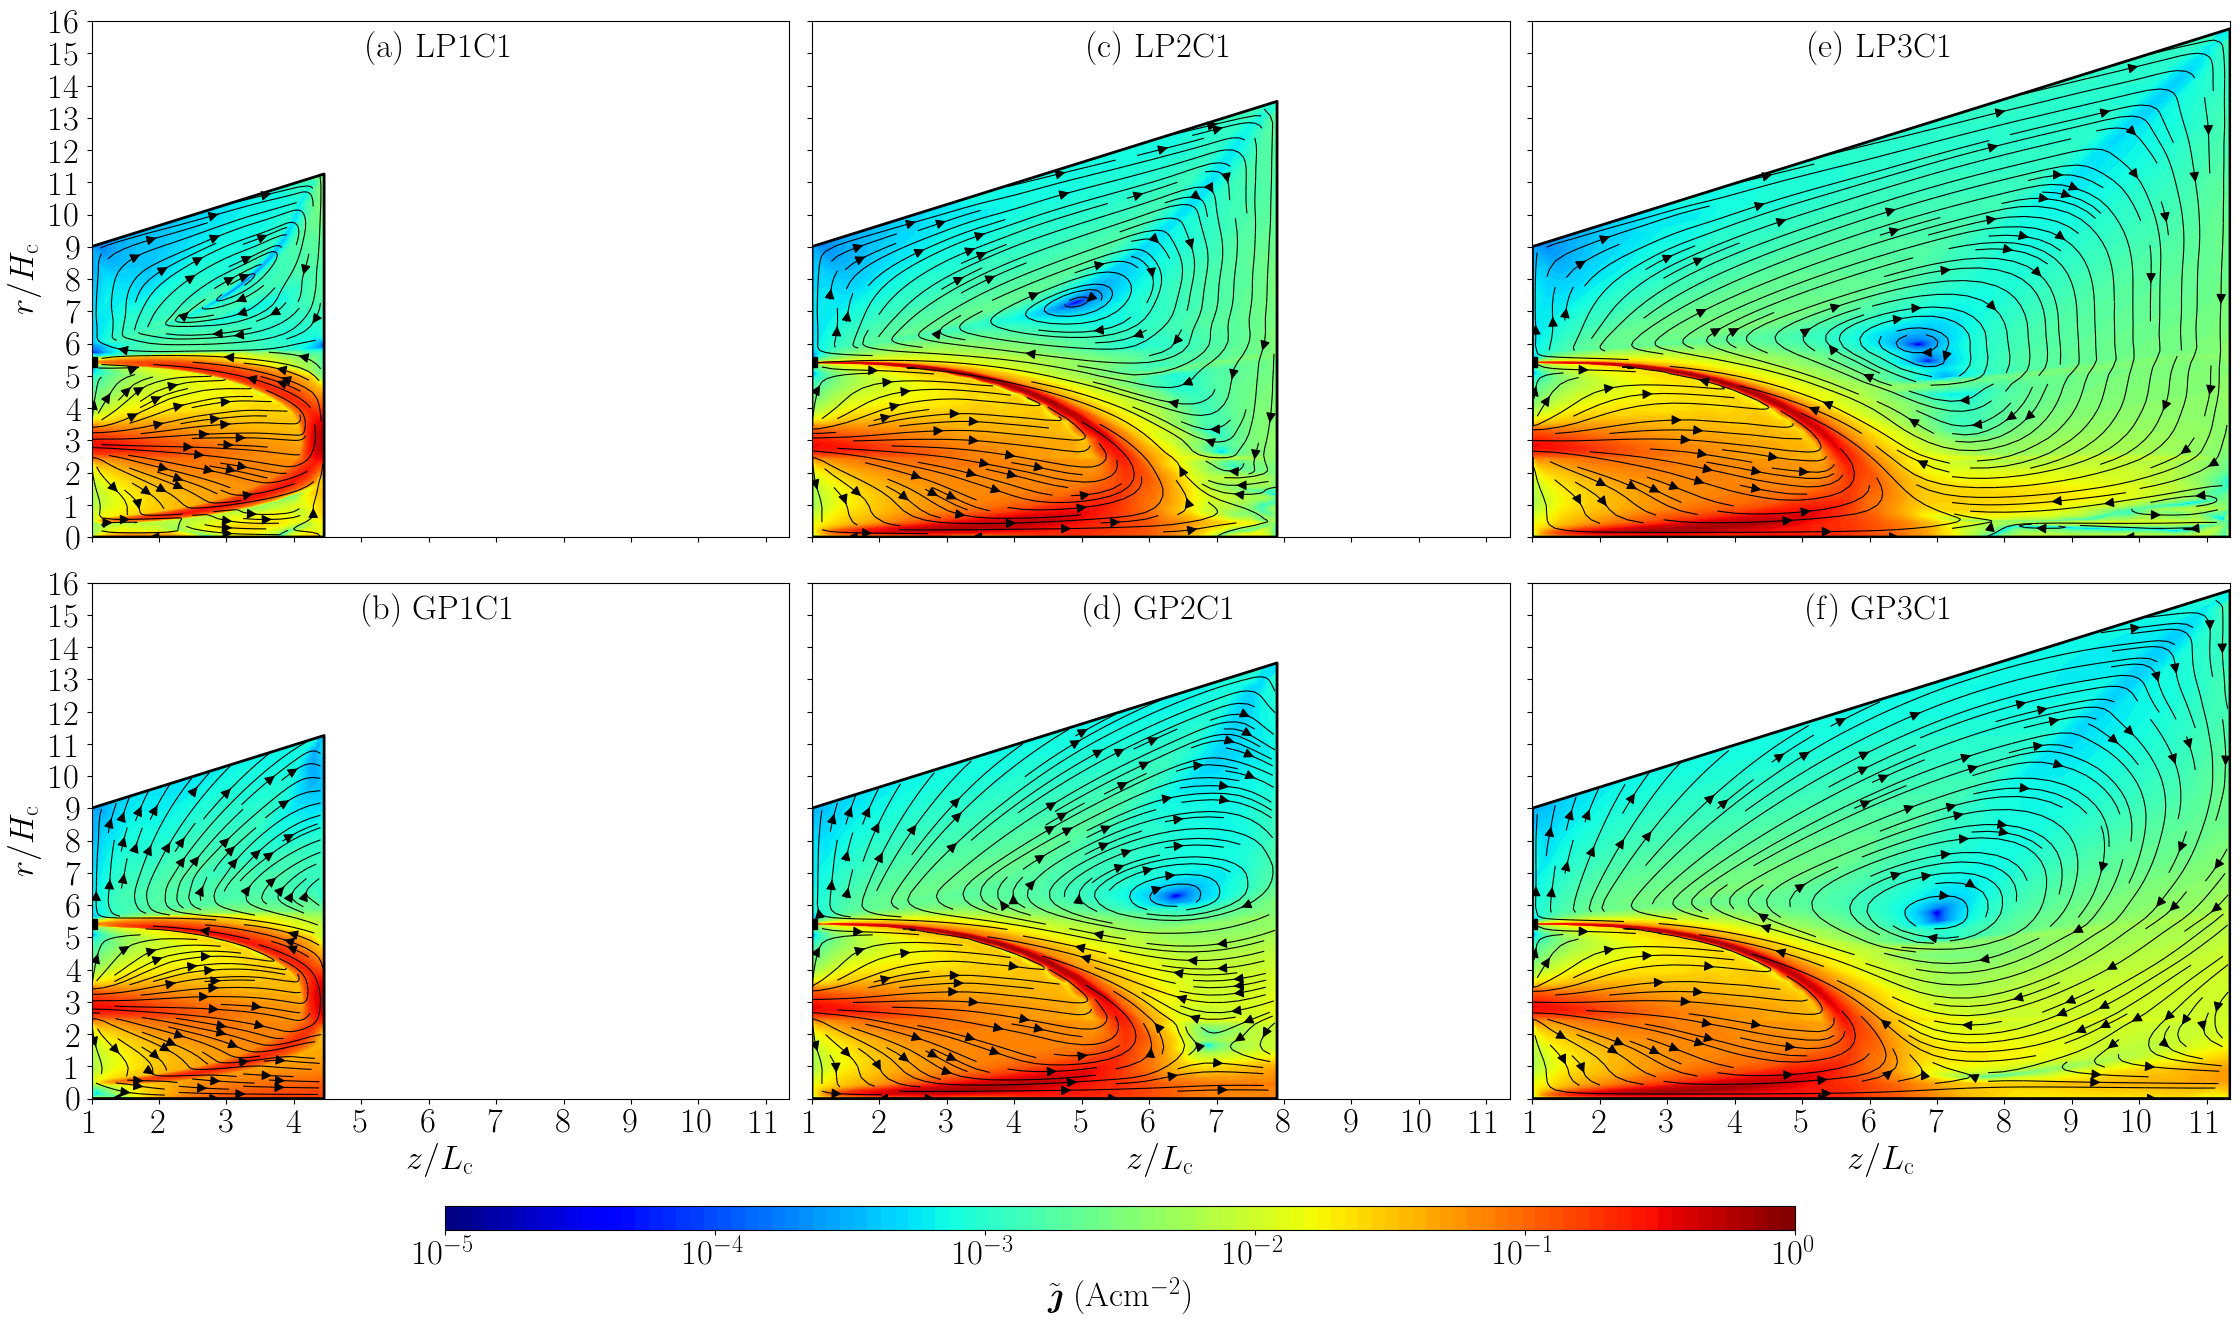
\includegraphics[width=1\textwidth]{figures/fig2.png}
\caption{
Plume sizes P1-P3 with C1 (the black square marker at $z/L_\mathrm{c}=1$) and with LPC (top row) and GPC (bottom row). 2D ($z$,$r$) contour maps and streamlines of $\tilde {\bm  \jmath}$.}
\label{fig: j_comp_P1P4}
\end{figure*}
%%%%%%%%%%%%%%%%%%%%%%%%%%%%%%%%%%%%%%%%%%%%%%%%%%%%%

%%%%% FIGURE 3: 2D maps of ji, je %%%%%%%%%%%%%%%%%%%
\begin{figure*}[!t]
\centering
\includegraphics[width=1\textwidth]{figures/fig3.pdf}
\caption{
2D ($z$,$r$) contour maps of (a) $\tilde {\bm  \jmath}_\mathrm{i}$ and (b) $\tilde {\bm  \jmath}_\mathrm{e}$ for case GP3C1, and (c) $\tilde {\bm  \jmath}_\mathrm{e}$ for case LP3C1. The black lines with arrows depict streamlines of $\tilde {\bm  \jmath}_\mathrm{i}$ in (a) and $-\tilde {\bm  \jmath}_\mathrm{e}$ in (b) and (c). Magenta lines indicate magnetic lines. The black square marker at $z/L_\mathrm{c}=1$ indicates the location of cathode C1.
}
\label{fig: P2_jemaps}
\end{figure*}
%%%%%%%%%%%%%%%%%%%%%%%%%%%%%%%%%%%%%%%%%%%%%%%%%%%%%%%%%%%


Differences on $\tilde{\bm\jmath}$ among cases are thus due quasi exclusively to $\tilde{\bm\jmath}_\mathrm{e}$. Figs. \ref{fig: P2_jemaps}(b) and \ref{fig: P2_jemaps}(c) show this current for cases GP3C1 and LP3C1, respectively.
%
For the two cases, the center of the electron beam travels along the CML. The component of this beam closest to the MS diffuses towards it and then exits outwards, primarily near the magnetic singular point, to neutralize the ion beam.
%
The main difference between the LPC and the GPC is found in the electron flow towards the lateral plume boundary.
%
The LPC promotes electron detachment from the magnetic lines, yielding a higher electron current towards the lateral plume boundary to locally cancel the ion current there (mainly carried by high-divergence fast ions and slow CEX ions). 
In contrast, the GPC reduces the electron current towards the lateral plume boundary, and the resulting electron streamlines follow more closely the local magnetic field lines, exhibiting a more progressive outward detachment towards the lateral boundary.
%
This solution is more representative of the still well-magnetized electron population in the simulated plume region: the surface-averaged values over the boundary P of the magnetic strength and the effective Hall parameter
are 7.4-1.8 G and 212.2-68.1, respectively, for plume sizes P1 to P4. 


Even though the electron current density at the lateral plume boundary is relatively low, on the order of 10$^{-5}$ to 10$^{-3}$ Acm$^{-2}$, the difference in lateral electron flow between the LPC and the GPC is physically relevant: in case GP3C1, approximately 10\% of $|I_\mathrm{eP}| \, (= I_\mathrm{iP})$ is collected at the lateral plume boundary, whereas this fraction increases to 14\% in case LP3C1. 
%
This result is in line with the simulations using the LPC reported in Ref. \citenum{orte16}, where the authors note that if the plume boundaries are set too close to the channel exit, the transport of electrons in the near plume gets perturbed by the zero local current condition, and more electron current across magnetic field lines may occur.
%
Electron detachment near the plume boundary has also been observed in HYPHEN simulations of an electrodeless plasma thruster with a MN, where the LPC was used \cite{zhou22a}.




%%%%% FIGURE 4: 1Ds profiles for P3 %%%%%%%%%%%%%%%%%%%
\begin{figure}[!t]
\centering
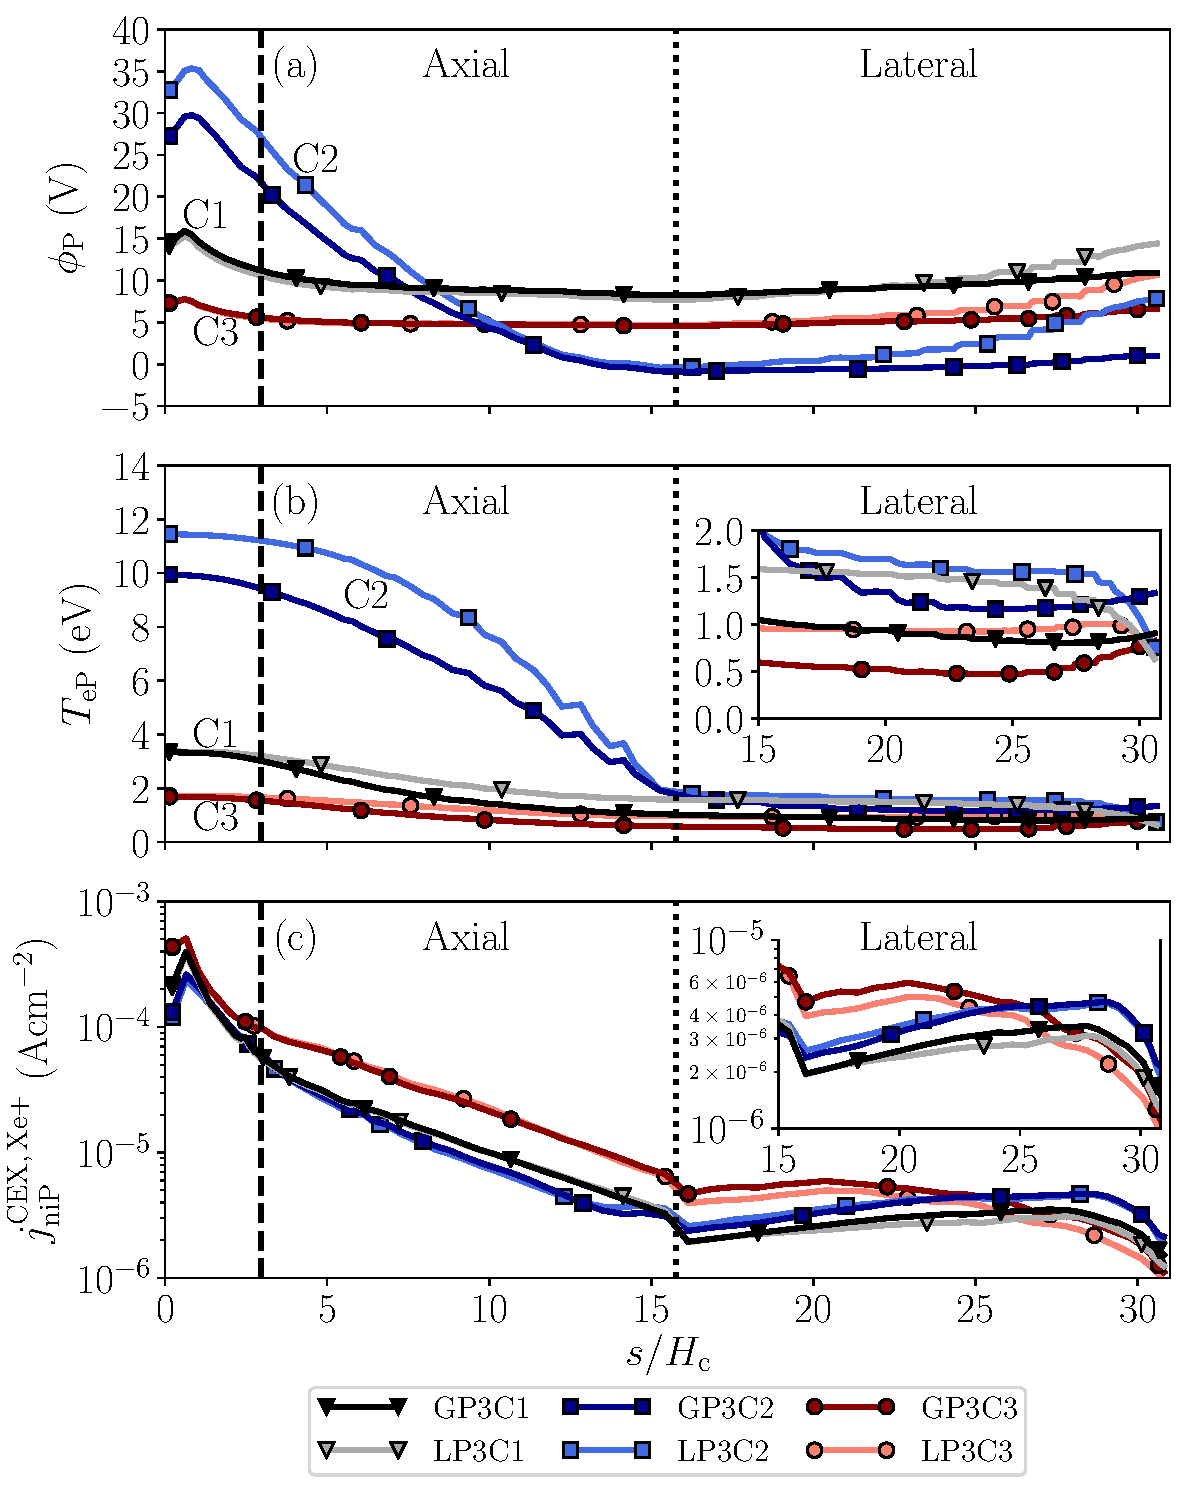
\includegraphics[width=1.0\columnwidth]{figures/fig4.pdf}
\caption{
Plume size P3. Comparison of profiles along P for the GPC and LPC. (a) $\phi_\mathrm{P}$, (b) $T_\mathrm{eP}$ and (c) the current density of singly charged slow CEX ions $j_\mathrm{niP}^\mathrm{CEX, Xe+}$. Coordinate $s$ runs along P with $s = 0$ at the symmetry axis. The vertical black dashed and dotted lines correspond to the thruster channel midradius and the upper-right corner of the plume domain, respectively.}
\label{fig: P2_down_1}
\end{figure}
%%%%%%%%%%%%%%%%%%%%%%%%%%%%%%%%%%%%%%%%%%%%%%%%%%%%%%%%%%%


%%%%% FIGURE 5: 1Dz profiles %%%%%%%%%%%%%%%%%%%%%%%%%%%%%%
\begin{figure*}[!t]
\centering
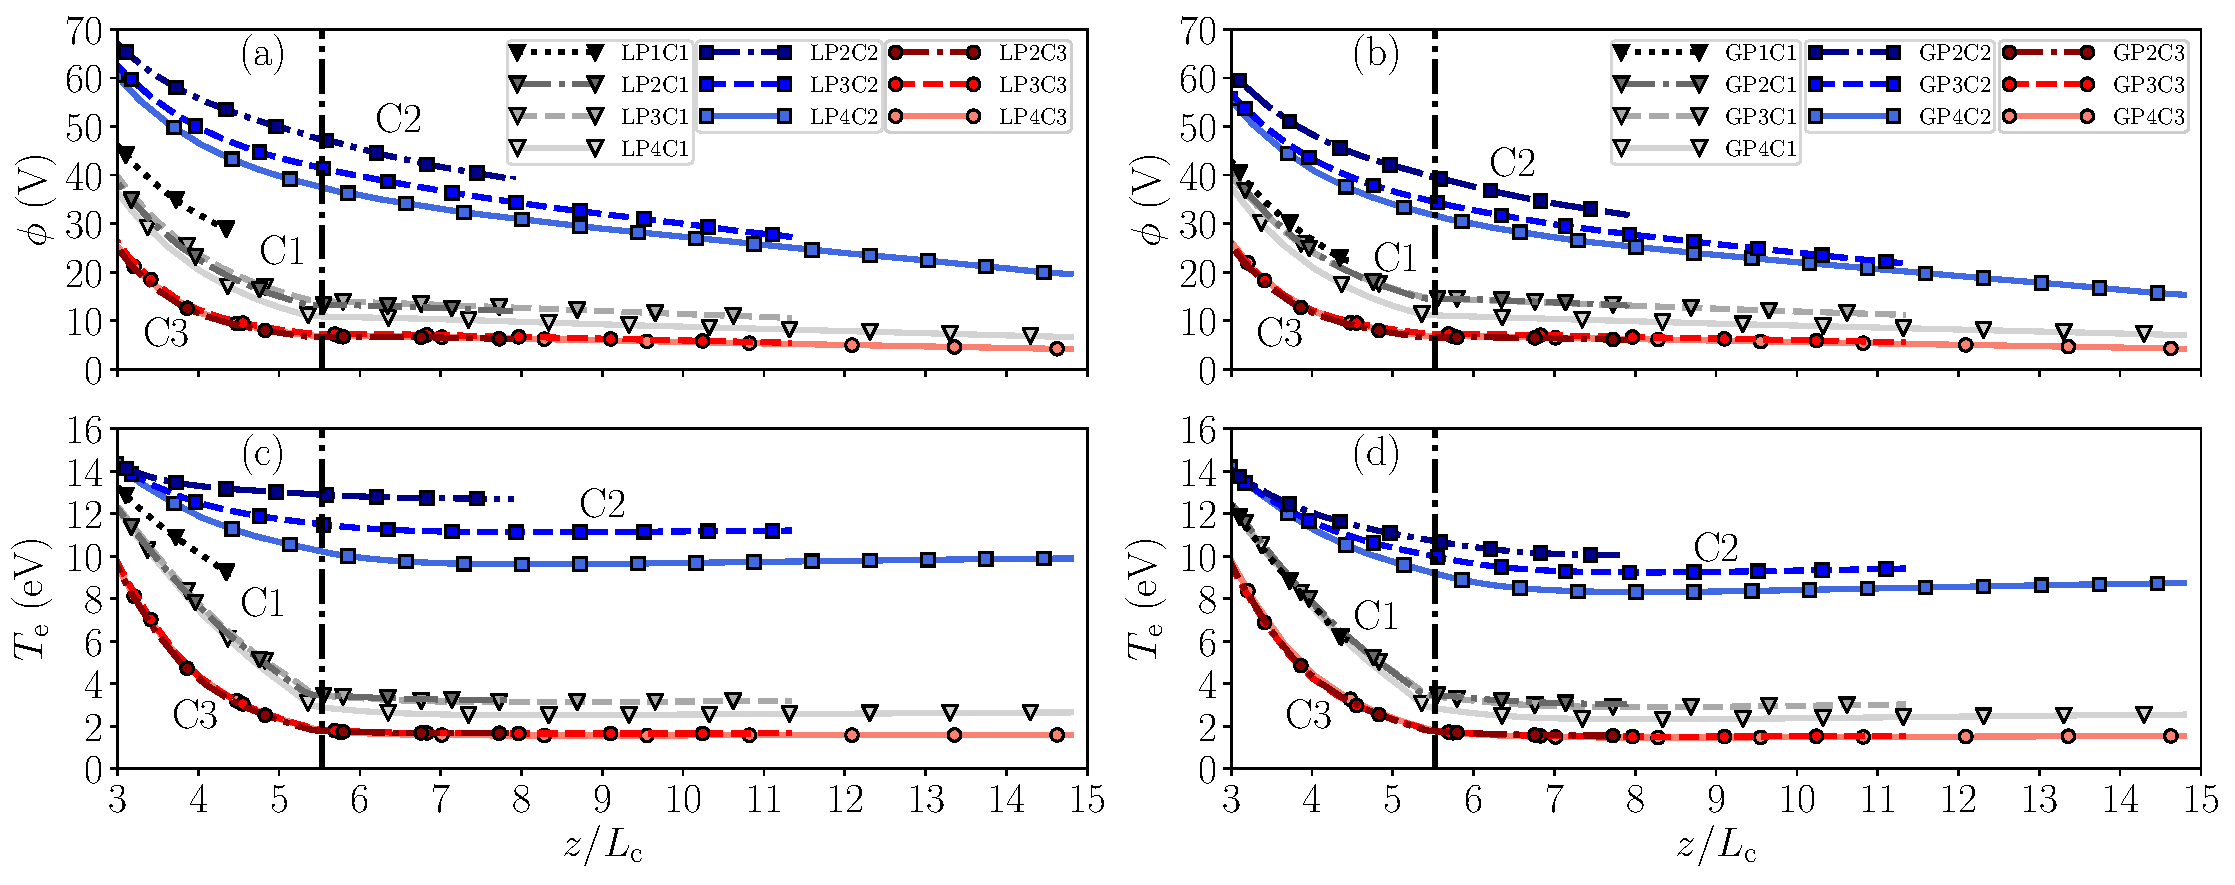
\includegraphics[width=1.0\textwidth]{figures/fig5.pdf}
\caption{
1D axial profiles along the thruster channel midline in the near-plume region for cases with the LPC (left column) and the GPC (right column). The vertical black dot-dashed line indicates the crossing point with the MS at $z/L_\mathrm{c} = 5.5$.
} 
\label{fig: 1Dz_comp_P1P4}
\end{figure*}
%%%%%%%%%%%%%%%%%%%%%%%%%%%%%%%%%%%%%%%%%%%%%%%%%%%%%%%%%%%

Fig. \ref{fig: P2_down_1} compares relevant plasma variables at the plume boundary P for all cases and plume size P3. The spatial variable runs first along the axial boundary, from the axis to the upper-right corner, and then continues from there up to $z/L_\mathrm{c} = 1$, along the lateral boundary [refer to Fig. \ref{fig: domain_meshes}(b)]. We focus now on the results for C1 cases. 
%
Figs. \ref{fig: P2_down_1}(a) and \ref{fig: P2_down_1}(b) show the electric potential and the electron temperature profiles, respectively.
%
Compared to case GP3C1, the larger electron current at the lateral plume boundary in case LP3C1 leads to an increase in $\phi_\mathrm{P}$ of up to approximately 30\% in that region. These differences in $\phi_\mathrm{P}$ between cases are on the order of the local $T_e$ and are therefore significant for near-plume diagnostics.
%
The electron temperature also exhibits non-negligible differences between the two cases, with lower values for case GP3C1 along most of the plume boundary. In particular, at the lateral boundary, $T_\mathrm{eP}$ in LP3C1 is up to about 70\% higher than in GP3C1.
%
An added value of the GPC is that the average energy deposited at P by exiting electron, $\mathcal{E}_\mathrm{neP} = -eP''_\mathrm{neP}/j_\mathrm{neP}$, is computed from Eq. \eqref{eq: energy_flux_P} yielding values ranging from 4.0$T_\mathrm{eP}$ to 9.2$T_\mathrm{eP}$ for case GP3C1, whereas the LPC sets it ``arbitrarily'' to 4.5$T_\mathrm{eP}$. According to Eq. \eqref{eq: energy_flux_P}, this implies that $e\phi_\mathrm{\infty P}/T_\mathrm{eP} \approx$ 2.0-7.2 for case GP3C1.



Fig. \ref{fig: P2_down_1}(c) compares the current density profiles at P of singly charged CEX ions, $j_\mathrm{niP}^\mathrm{CEX, Xe+}$. The differences in $\phi_\mathrm{P}$ at the lateral plume boundary between GP3C1 and LP3C1 cases affect the dynamics of CEX ions. In particular, the higher $\phi_\mathrm{P}$ in case LP3C1 reduces $j_\mathrm{niP}^\mathrm{CEX, Xe+}$ by up to 16\%, while increasing the average energy of these ions at P (not shown) by up to 11\%.
%
Although, as previously discussed, CEX ions constitute a minor population in the plume (contributing only about 1\% to the fraction of $I_\mathrm{iP}$ through the lateral plume boundary) their accurate characterization is essential for assessing plume–satellite interaction effects.




Fig. \ref{fig: 1Dz_comp_P1P4} shows the axial profiles of $\phi$ and $T_\mathrm{e}$ along the channel midline for $z/L_\mathrm{c} \geq 3$, for the LPC (left) and the GPC (right) models, the different plume sizes and cathode locations. The plasma density $n_\mathrm{e}$ is very similar for all cases and was not plotted. Also, for $z/L_\mathrm{c} < 3$ (not shown), all cases present very similar profiles for all variables, with peak values $T_\mathrm{e} \approx 28$ eV and $n_\mathrm{e} \approx 1.7\cdot 10^{18}$ m$^{-3}$. 
Focusing now only on C1 cases, the results show only moderate relative variations on $\phi$ and $T_\mathrm{e}$ along the channel midline across cases (especially for sizes P2-P4), despite the significant differences observed in the plasma current maps and in $\phi$ and $T_\mathrm{e}$ at the lateral plume boundary, as discussed above. 



Tab. \ref{tab: F_Id 2} lists the main performance figures for the eight simulation cases of C1, beginning with the cathode coupling voltage, $V_\mathrm{cc}$.
For plume size P1, $V_\mathrm{cc}$ values correspond to the electric potential at the plume boundary at the channel midradius.
For plume sizes P2-P4, $V_\mathrm{cc}$ is estimated as the electric potential value at the crossing point between the channel midline and the CML \cite{jorn21}.
For both the LPC and GPC, the largest differences in $V_\mathrm{cc}$ are found for plume size P4.
%
As noted in Sec. \ref{sec: sim_settings}, these discrepancies result from minor variations on the CML due to the nontrivial optimization of the MFAM cell layout for each plume domain, and do not reflect any significant physical change in the cathode-beam coupling process.
Mesh-related variations in $V_\mathrm{cc}$ have been quantified to be approximately $\pm 3$ V.
%
Nonetheless, the largest differences in $V_\mathrm{cc}$ across P2-P4 cases are on the order of 1\% of $V_\mathrm{d}$.
This indicates a very similar effective ion acceleration in the discharge for all cases,
%
which is in line with the very small differences (below 2\%) observed in the thrust, $F$, among cases, as listed in Tab. \ref{tab: F_Id 2}. The values of $F_\mathrm{e}$ and $F_\mathrm{i}$ correspond to the contributions to thrust (i.e., the downstream axial momentum fluxes) from the electron and ion species, including CEX populations.  The contribution to thrust from neutral species remains approximately 1 mN across all cases. As expected, electron momentum flux is transferred to ion momentum flux as the plasma beam moves downstream. The small increase (on average) in thrust with the plume size is due to the small magnetic force over the plasma there. It is assumed that the residual magnetic force between P and infinity has a negligible impact in thrust. 

An important asset of the GPC is the determination of the potential at infinity, $\phi_\infty$, also given in Tab. \ref{tab: F_Id 2} for the four plume sizes.
%
For sufficiently large plumes, i.e., plume sizes P2-P4, $\phi_\infty$ monotonically decreases with the plume size. The total decrease from P2 to P4 amounts to about 78\% of its value for P2: 30\% from P2 to P3 and 48\% from P3 to P4. This suggests that simulating a plume size larger than P4 would be necessary for a precise estimation of $\phi_\infty$. However, the results indicate that increasing the plume size leads to only incremental variations in $\phi$ along the thruster channel midline
and $F$, and thus the effect on discharge performance is minimal. Moreover, the quality of the MFAM tends to deteriorate significantly for very large plumes. Mesh-related variations in $\phi_\infty$ are lower than those stated before for $V_\mathrm{cc}$, and amount to just $\pm 1$ V, approximately.



%%%%% TABLE 2: C1 %%%%%%%%%%%%%%%%%%%%%%%%%%%%%%%%%%%%%%%%%
\begin{table}[!t]
\centering
\resizebox{1.0\columnwidth}{!}{
{\renewcommand{\arraystretch}{1.0}
\begin{tabular}{|c||c|c|c|c||c|c|c|c|}
\hline
& GP1C1 & GP2C1 & GP3C1 & GP4C1 & LP1C1 & LP2C1 & LP3C1 & LP4C1 \\ \hline \hline
$V_\mathrm{cc}$ (V) & 21.39 & 14.52 & 14.90 & 11.39 & 26.00 & 13.21  & 13.98  & 11.07 \\ \hline
$\phi_\infty$ (V)    & 5.80  & 6.17  & 4.31  & 1.33  & N/A   & N/A   & N/A   & N/A   \\ \hline
$F$ (mN)             & 280.1 & 284.0 & 283.9 & 286.5 & 279.6 & 286.0 & 284.8 & 286.1 \\ \hline
$F_\mathrm{i}$ (mN)  & 274.7 & 280.6 & 281.1 & 284.4 & 272.3 & 282.3 & 281.9 & 284.0 \\ \hline
$F_\mathrm{e}$ (mN)  & 4.3   & 2.4   & 1.7   & 1.0   & 6.3   & 2.8   & 1.9   & 1.0   \\ \hline
$\eta$               & 0.39  & 0.40  & 0.40  & 0.41  & 0.39  & 0.40  & 0.40  & 0.41  \\ \hline
$\eta_\mathrm{ene}$  & 0.65  & 0.64  & 0.65  & 0.65  & 0.65  & 0.64  & 0.64  & 0.65  \\ \hline
$\eta_\mathrm{div}$  & 0.77  & 0.78  & 0.79  & 0.77  & 0.77  & 0.78  & 0.78  & 0.78  \\ \hline
$\eta_\mathrm{disp}$ & 0.78  & 0.80  & 0.78  & 0.81  & 0.78  & 0.80  & 0.80  & 0.80  \\ \hline
\end{tabular}
}
}
\caption{
Performance figures for plume sizes P1 to P4 with C1 and the GPC and LPC.
}
\label{tab: F_Id 2}
\end{table}
%%%%%%%%%%%%%%%%%%%%%%%%%%%%%%%%%%%%%%%%%%%%%%%%%%%%%%%%%%%



The global plasma power balance is detailed in Eq. \eqref{eq: power_balance} of the Appendix \ref{sec: App balances} and shows only small variations (below 2\%) in its different contributions across cases. 
%
The discharge current, $I_\mathrm{d}$, is practically the same for all cases, and approximately equal to 17.84 A, with maximum differences of about 1\%. Therefore, for all cases the total power deposited into the plasma is $P \simeq V_\mathrm{d}I_\mathrm{d} \approx 5.4$ kW, and the thrust efficiency is $\eta = F^2/(2\dot{m}P) \approx 40\%$.
%
According to Eq. \eqref{eq: thrust efficiency}, $\eta$ is conveniently factored as the product of three partial efficiencies, which are defined in Eq. \eqref{eq: partial_eff1}: the energy efficiency, $\eta_\mathrm{ene}$, which represents the fraction of the total power deposited into P; the divergence efficiency, $\eta_\mathrm{div}$; and the dispersion efficiency, $\eta_\mathrm{disp}$. The latter two partial efficiencies are plume-related metrics that assess plume divergence and velocity dispersion, respectively.
These partial efficiencies, listed in Tab. \ref{tab: F_Id 2}, also show slight changes (maximum 3\%) between cases. (Note that  we aim to highlight here that the differences between cases are minimal and not the values themselves.)


Therefore, for a cathode located inside or at the MS, and provided that the size of the simulated plume region is sufficiently large such that $\phi$ variations in the downstream part of the plume are much smaller than $V_\mathrm{d}$, we conclude that thruster performance is well determined regardless of whether the LPC or GPC is used. Nonetheless, it is evident that plume conditions significantly impact plasma current maps within the plume and the solution for $\phi$ and $T_\mathrm{e}$ in the lateral part of the plume, which is important for plume characterization and comparison with experimental data (noting that the plume is the plasma region most accessible to diagnostics).

Finally, Figs. \ref{fig: 1Dz_comp_P1P4}(c) and \ref{fig: 1Dz_comp_P1P4}(d) reveal that for sizes P2-P4, $T_\mathrm{e}$ remains nearly constant at relatively low values, around 2.5 eV, downstream the MS, and no significant electron cooling is observed, in line with the results in Ref. \citenum{mike09}.
%
Previous kinetic studies on magnetized plumes have shown that the total potential fall to infinity in the plume is primarily determined by the electron thermal energy \cite{ahed20a}. 
%
Here, the surface-averaged value of $e\phi_\mathrm{\infty P}/T_\mathrm{eP}$ over P varies slightly with plume size, ranging between 4.7 and 5.7 
(which, taking $T_\mathrm{iP}/T_\mathrm{eP} \approx 10$, as obtained here, agrees very well with simulations for a MN in Ref. \citenum{ahed20a}).
Since $T_\mathrm{eP}\sim$ 1eV,  $\phi_\mathrm{\infty P}$ still amounts to about 15-20\% of the potential drop in the near plume downstream of $z/L_\mathrm{c} = 3$.
%
Increasing plume size results in only a small decrease in $\phi_\mathrm{P}$ and the Hall parameter, but not in $T_\mathrm{eP}$. This suggests that anomalous parallel-field electron cooling \cite{zhou21a} should be considered in the MN region of the plume, similar to the approach taken for electrodeless plasma thruster simulations with HYPHEN in Ref. \citenum{zhou22a}.



%%%%%%%%%%%%%%%%%%%%%
\section{Influence of cathode location on current maps and cathode coupling}\label{sec: cathode location}
%%%%%%%%%%%%%%%%%%%%%   

This section analyzes the effects of cathode configuration on key plasma parameters in the plume, including maps of electric and electron currents, electric potential, electron temperature, the cathode coupling voltage, and the main performance figures. We show that the trends observed in these plasma parameters are in good agreement with previous numerical and experimental studies.
%
The cathode configurations described in Sec. \ref{sec: sim_settings} are considered. We begin by showing that, for C2 cases (i.e., a laterally-mounted cathode located outside the MS), LPC results are strongly affected by plume size and are thus unreliable. Therefore, the remainder of the discussion focuses on GPC cases.


Figs. \ref{fig: j_and_je_cath}(a)-(d) show $\tilde{\bm\jmath}$ for C2 cases with plume sizes P3 and P4. 
%
As discussed in Secs. \ref{sec: sim_settings} and \ref{sec: comp_local_GDML}, for plume sizes P2-P4 and C1, the CML is enclosed by the MS (blue dashed line in Fig. \ref{fig: j_and_je_cath}), forming a closed loop within the simulated plume domain, which is located sufficiently far from the P boundary.
%
In contrast, for C2 cases, the CML (red dashed line in Fig. \ref{fig: j_and_je_cath}) extends downstream along the plume and intersects the P boundary. The anode-to-cathode current loop closes downstream of the MS, below the CML, and a second counter-rotating current loop forms above the CML.
%
When the LPC is applied, current streamlines of these two counter-rotating current loops are constrained to be parallel to the P boundary, so that they must necessarily converge at a plasma stagnation point at P featuring $\tilde{\boldsymbol{\jmath}}=0$. Therefore, the current solution provided by the LPC is inherently dependent on the plume size: observe in Figs. \ref{fig: j_and_je_cath}(a) and (c) how, for cases LP3C2 and LP4C2, this point moves with the downstream boundary of the plume, and the electric current loops in the near plume exhibit notable differences in the region common to both cases.
%
On the other hand, by locally decoupling ion and electron currents at P, the GPC allows these current loops to close \textit{at infinity}. As a result, the influence of the P boundary on the current solution is significantly reduced, making it more robust to variations in plume size.
In particular, the plasma stagnation point at P, which is induced artificially by the LPC, is absent when the GPC is applied. Instead, a $\tilde{\boldsymbol{\jmath}}=0$ point appears within the domain, located at a similar position for both P3 and P4 sizes.

Figs. \ref{fig: j_and_je_cath}(e) and \ref{fig: j_and_je_cath}(f) show $\tilde{\bm\jmath}_\mathrm{e}$ for cases LP4C2 and GP4C2, respectively. 
%
The central part of the electron beam emitted by cathode C2 travels downstream along the CML and yields a local maximum in the $\tilde{\bm\jmath}_\mathrm{e}$ magnitude near the upper-right corner of the plume domain, where the CML intersects the P boundary.
%
Now, only the fraction of electrons emitted by the cathode closest to the MS travels along it towards the singular point, where they penetrate into the interior region of the separatrix and subsequently into the thruster channel.
%
This behavior has also been observed in three-dimensional hybrid simulations of the near plume of a HET with a similar magnetic topology, when the cathode is placed in the lateral region of the plume, outside the MS \cite{cich21a}.

Fig. \ref{fig: j_and_je_cath_3} shows $\tilde{\bm\jmath}$ and $\tilde{\bm\jmath}_\mathrm{e}$ maps for C3 cases with plume size P3 (as in C1 cases, results for size P4 are similar with both the GPC and LPC and are therefore omitted for simplicity). The solutions for $\tilde{\bm\jmath}$ and $\tilde{\bm\jmath}_\mathrm{e}$ downstream of the MS closely resemble those found for C1 cases, as described in Sec. \ref{sec: comp_local_GDML}. The main differences compared to C1 cases arise in the anode-to-cathode current loop inside the MS: the centrally-mounted cathode generates significantly higher local $\tilde{\bm\jmath}$ and $\tilde{\bm\jmath}_\mathrm{e}$ in the cathode near-plume along the axis and enhances the coupling between cathode electrons and the ion beam exiting the thruster channel (see later). This improvement occurs because the outermost component of the electron beam emitted from the cathode diffuses towards the thruster exit plane well upstream of the MS, prior to reaching it.

As in C1 cases, BCs and plume size have minimal impact on $\tilde{\bm\jmath}_\mathrm{i}$ for C2 and C3 cases (maps are omitted for brevity). The main effect of cathode location appears in the ion divergence, as discussed later.
%
Therefore, the differences in $\tilde{\bm\jmath}$ stem primarily from variations in $\tilde{\bm\jmath}_\mathrm{e}$ induced by the plume condition, following the same trend as in C1 cases: compared to the GPC, the LPC promotes electron detachment from magnetic lines, leading to a higher electron current towards the lateral plume boundary [compare Figs. \ref{fig: j_and_je_cath}(e) and \ref{fig: j_and_je_cath}(f) for C2, and Figs. \ref{fig: j_and_je_cath_3}(c) and \ref{fig: j_and_je_cath_3}(d) for C3].
%
As discussed in Sec. \ref{sec: comp_local_GDML} for C1 cases, this yields higher $\phi_\mathrm{P}$ (and $T_\mathrm{eP}$) values at the lateral plume boundary [refer to Figs. \ref{fig: P2_down_1}(a) and \ref{fig: P2_down_1}(b)]. The differences between the LPC and GPC are larger (smaller) in C2 (C3) cases, respectively, and relevant for plume diagnostics in all cases. Additionally, there is a comparable influence on the current density of CEX ions at the lateral part of the plume boundary [see Fig. \ref{fig: P2_down_1}(c)].
%
%
Given the strong impact of plume size on the current solution in C2 cases when the LPC is applied, the following analysis focuses exclusively on GPC cases.




%%%%% FIGURE 6: 2D maps of j and je for C2 %%%%%%%%%%%%%%%%
\begin{figure*}[!pht]
\centering
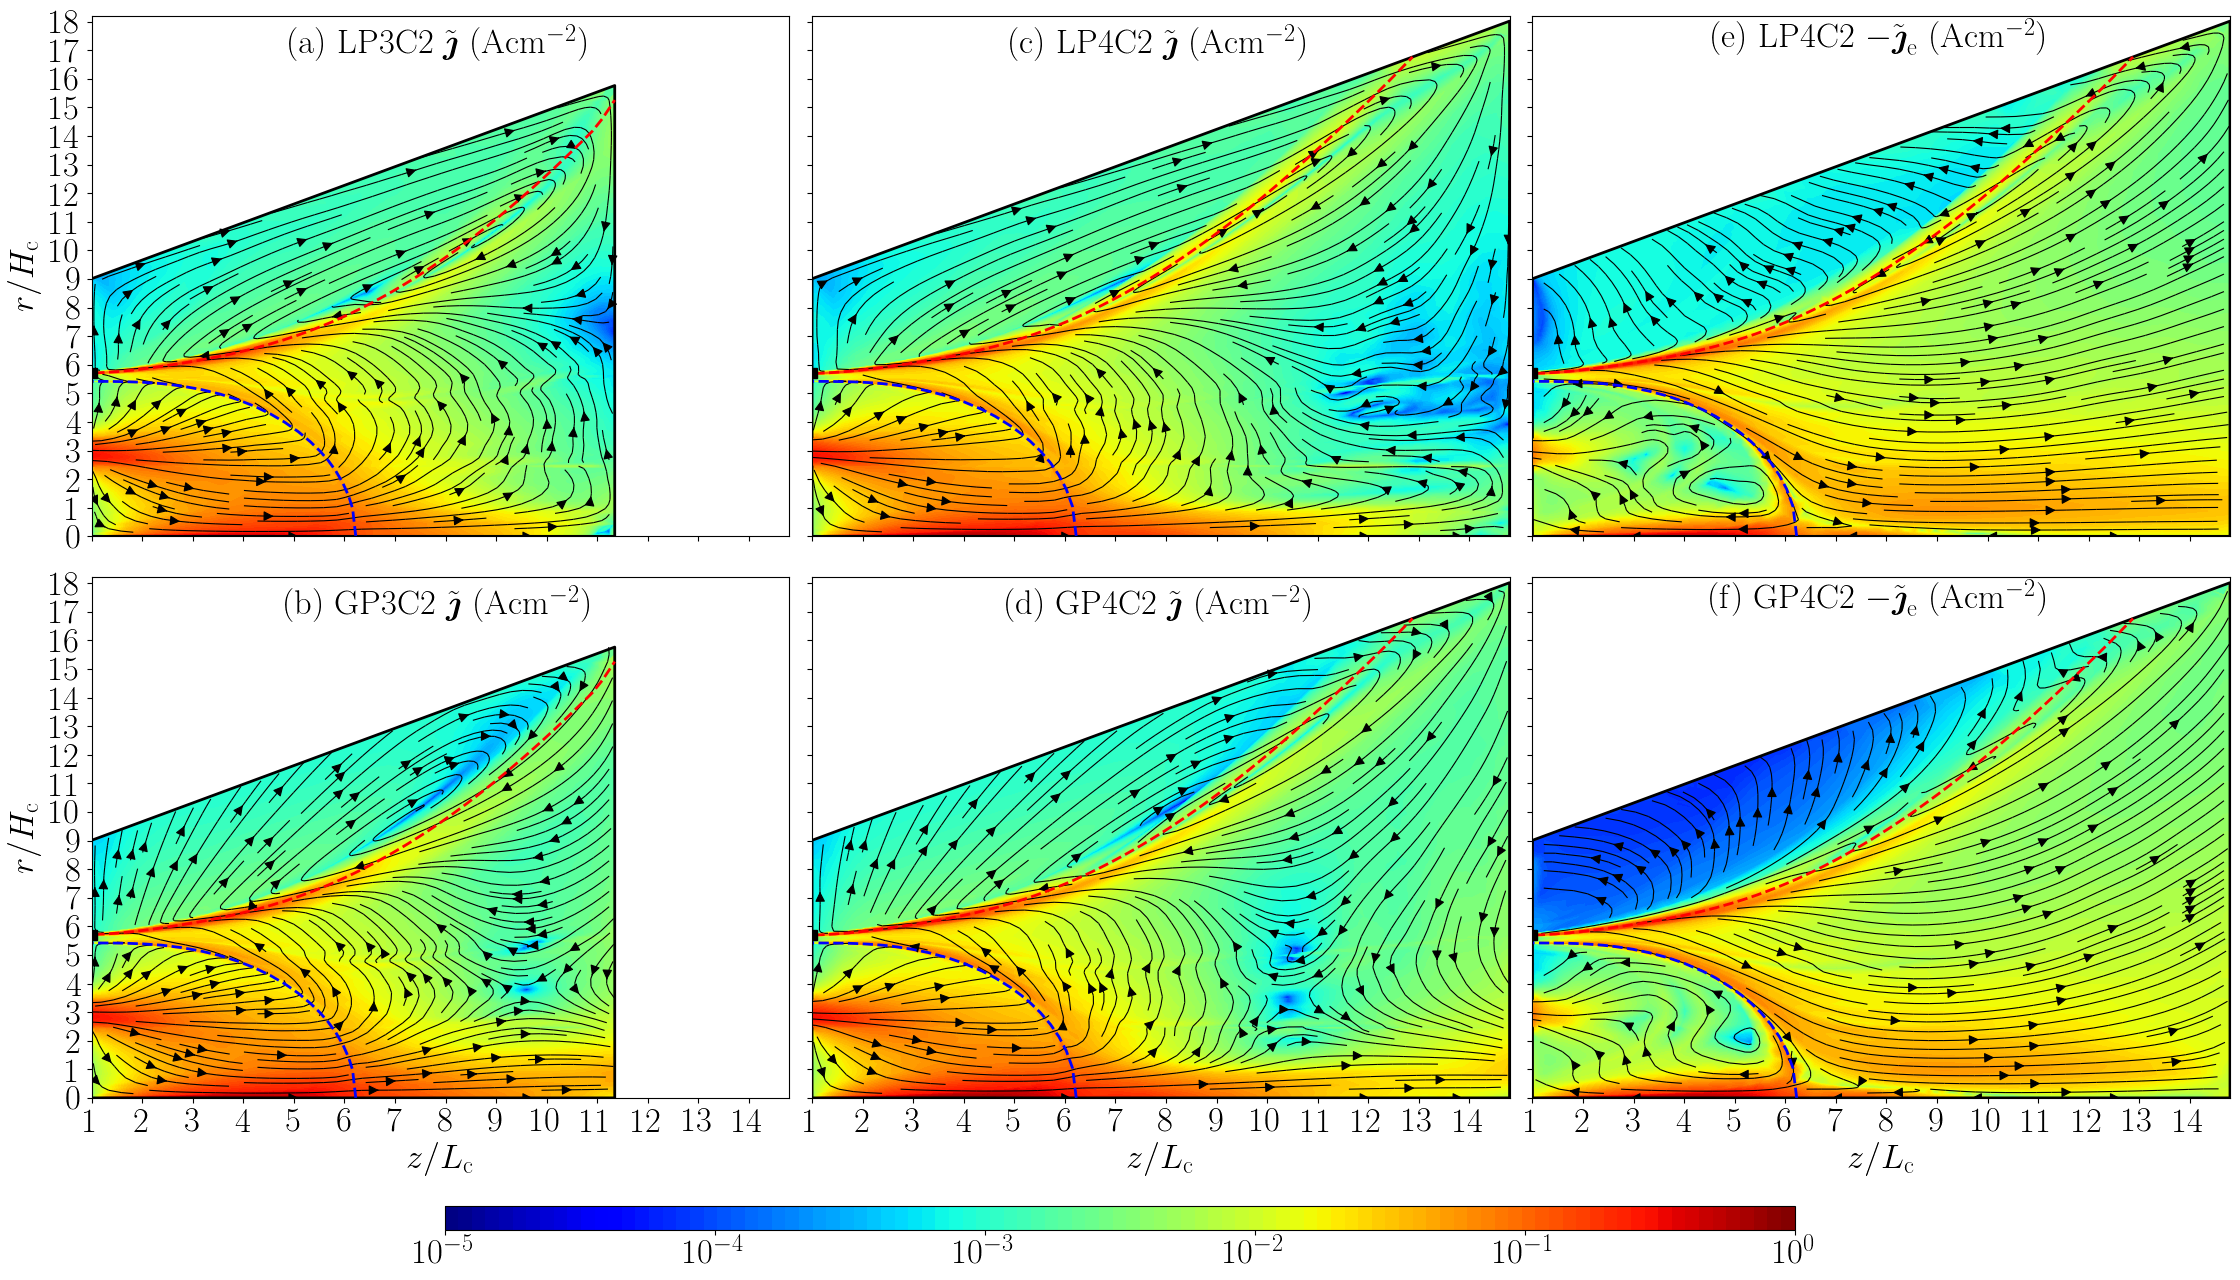
\includegraphics[width=1\textwidth]
{figures/fig6.png}
\caption{
Plasma plume maps when using the lateral MS-external cathode C2 (the black square marker at $z/L_\mathrm{c}=1$). Top and bottom rows are for the LPC and GPC models, respectively. (a)-(d) 2D maps of $\tilde {\bm  \jmath}$ for plume sizes P3 and P4, and (e)-(f) 2D maps of $\tilde {\bm  \jmath}_\mathrm{e}$ for plume size P3. In all plots, the red and blue dashed lines correspond to the CML and the MS, respectively.
}
\label{fig: j_and_je_cath}
\end{figure*}
%%%%%%%%%%%%%%%%%%%%%%%%%%%%%%%%%%%%%%%%%%%%%%%%%%%%%%%%%%%

%%%%% FIGURE 7: 2D maps of j and je for C3 %%%%%%%%%%%%%%%%
\begin{figure*}[!pht]
\centering
\includegraphics[width=0.62\textwidth]
{figures/fig7.pdf}
\caption{
Plasma plume maps when using the centrally-mounted cathode C3 (the black square marker at $z/L_\mathrm{c}=1$). Top and bottom rows are for the LPC and GPC models, respectively. The plume size P3 is used. (a)-(b) 2D maps of $\tilde {\bm  \jmath}$, and (c)-(d) 2D maps of $\tilde {\bm  \jmath}_\mathrm{e}$. In all plots, the blue dashed lines correspond to the off-axis MS.
}
\label{fig: j_and_je_cath_3}
\end{figure*}
%%%%%%%%%%%%%%%%%%%%%%%%%%%%%%%%%%%%%%%%%%%%%%%%%%%%%%%%%%%

%%%%% NEW TABLE 3: C2 and C3 GPC %%%%%%%%%%%%%%%%%%%%%%%%%%
\begin{table}[!t]
\centering
\resizebox{1.0\columnwidth}{!}{
{\renewcommand{\arraystretch}{1.0}
\begin{tabular}{|c||c|c|c||c|c|c|}
\hline
& GP2C2 & GP3C2 & GP4C2 & GP2C3 & GP3C3 & GP4C3 \\ \hline \hline
$V_\mathrm{cc}$ (V)  & 38.86 & 34.19  & 31.56  & 6.40 & 7.00  & 6.50 \\ \hline
$\phi_\infty$ (V)    & -4.95 & -12.75 & -14.78 & 2.65 & 2.10  & 0.74   \\ \hline
$F$ (mN)             & 271.4 & 272.1  & 275.2  & 297.1 & 294.9 & 296.6 \\ \hline
$F_\mathrm{i}$ (mN)  & 264.5 & 267.1  & 271.7  & 294.1 & 292.3 & 294.3 \\ \hline
$F_\mathrm{e}$ (mN)  & 6.0   & 4.1    & 2.6    & 1.6   & 1.1   & 0.7   \\ \hline
$\eta$               & 0.37  & 0.37   & 0.38   & 0.42  & 0.42  & 0.42  \\ \hline
$\eta_\mathrm{ene}$  & 0.70  & 0.69   & 0.71   & 0.64  & 0.64  & 0.64  \\ \hline
$\eta_\mathrm{div}$  & 0.71  & 0.70   & 0.71   & 0.80  & 0.80  & 0.79  \\ \hline
$\eta_\mathrm{disp}$ & 0.75  & 0.76   & 0.76   & 0.82  & 0.82  & 0.84  \\ \hline
\end{tabular}
}
}
\caption{
Performance figures for plume sizes P2 to P4 for C2 and C3 cases with GPC.
}
\label{tab: F_Id 2 cath}
\end{table}
%%%%%%%%%%%%%%%%%%%%%%%%%%%%%%%%%%%%%%%%%%%%%%%%%%%%%%%%%%%


We next examine the main performance figures for C2 and C3 cases, summarized in Tab. \ref{tab: F_Id 2 cath}.
%
For both C2 and C3 cases, $V_\mathrm{cc}$ is estimated as the electric potential at the crossing point between the channel midline and the MS. This choice enables a more consistent comparison with C1 cases, and it is also physically motivated. In C3 cases, the CML is the symmetry axis, and a large fraction of cathode-emitted electrons is guided near the MS towards the channel midline [see Fig. \ref{fig: j_and_je_cath_3}(d)].
%
In C2 cases, the component of the cathode-emitted electron flow that enters the thruster channel travels along the MS toward the magnetic singular point [refer to Fig. \ref{fig: j_and_je_cath}(f)].
%
Therefore, the MS serves as a meaningful reference magnetic surface for characterizing the coupling between cathode electrons and the ion beam.


We focus first on the effects of cathode location for any plume size (P2 to P4). Reducing the cathode radial position (i.e., moving from C2 to C1 to C3) results in lower $V_\mathrm{cc}$, and thus improved cathode-beam coupling, and higher values of both $F$ and $\eta$ (up to 5\% in absolute terms). Since $I_\mathrm{d}$ also increases (from 17.26 to 17.84 to 18.22 A, respectively), and thus $P \simeq V_\mathrm{d}I_\mathrm{d}$, the higher $\eta$ is attributed to the higher $F$.
%
Furthermore, partial efficiencies reveal an increase in $\eta_\mathrm{div}$ (up to 10\%) and $\eta_\mathrm{disp}$ (up to 8\%), indicating lower plume divergence and velocity dispersion, and a decrease in $\eta_\mathrm{ene}$ (up to 7\%).

Several experimental and numerical studies have reported results consistent with the behavior of $V_\mathrm{cc}$, $F$, $\eta$, and plume divergence observed here. 
%
For an laterally-mounted cathode, Ref. \citenum{till99} reported a decrease in thrust with increasing radial position of the cathode, leading to the conclusion that the optimal cathode position is as close as possible to the outer magnet pole.
%
Various experimental works have reported an increase in $V_\mathrm{cc}$ and poorer performance when increasing the radial position of the laterally-mounted cathode, in particular for locations outside the MS \cite{somm11b,tura16,yu17,ding18}.
%
Measurements on a HET with an laterally-mounted cathode and a magnetic topology lacking an off-axis separatrix indicated that $V_\mathrm{cc}$ increased in magnitude with the radial position of the cathode when the cathode was moved across regions of high electron magnetization, where the effective Hall parameter was about 500 \cite{frie16a}. Here, $V_\mathrm{cc}$ increases with the radial position of the cathode, i.e., moving from C3 to C1 to C2, being the corresponding effective Hall parameter in the cathode region about 52, 215 and 350, respectively.
%
For a 6 kW HET, Jameson \textit{et al.} \cite{jame07} compared the performance with externally and centrally-mounted (i.e., on-axis) cathodes. Higher $V_\mathrm{cc}$ values were observed when operating with the laterally-mounted cathode, while efficiency was reported to increase by 2-3\% when using the centrally-mounted cathode.
%
Compared to the operation with an laterally-mounted cathode, reduced $V_\mathrm{cc}$ and plume divergence were also reported in Ref. \citenum{hofe08b} for a 8 kW HET with a centrally-mounted cathode. Full PIC 2D axial-radial simulations \cite{cho17,cao20} have captured the lower plume divergence found in experiments when operating with a centrally-mounted cathode. 


On the other hand, the higher the radial position of the cathode, the more pronounced the variations in all performance figures with plume size. The value of $\phi_\infty$ decreases with increasing plume size for all cathode positions, with C2 (C3) cases exhibiting the largest (smallest) variations, respectively. This behavior suggests that simulating sufficiently large plume domains is particularly important when the cathode is located outside the MS.


We focus now on the solutions for $\phi$ and $T_\mathrm{e}$ in the plume.
%
First, the results in Figs. \ref{fig: 1Dz_comp_P1P4}(b) and \ref{fig: 1Dz_comp_P1P4}(d) reveal a higher impact of plume size when the cathode is placed at larger radial positions: the axial profiles practically collapse for C3 cases, whereas the largest variations are found among C2 cases.
%
Second, for any plume size, Figs. \ref{fig: 1Dz_comp_P1P4}(b) and \ref{fig: 1Dz_comp_P1P4}(d) show that $\phi$ and $T_\mathrm{e}$ along the channel midline increase with the radial position of the cathode (i.e., moving from C3 to C1 to C2). The plasma density, $n_\mathrm{e}$, in the plume (not shown) is found to decrease from C3 to C1, and remain approximately constant from C1 to C2.
%
Third, for case GP3C2, Fig. \ref{fig: P2_down_1}(a) reveals higher $\phi_\mathrm{P}$ values near the axis and the midradius along the axial plume boundary, and lower values along the lateral plume boundary. This results in a higher radial electric field in the plume (not shown), which is the primary responsible for the higher plume divergence and velocity dispersion of C2 cases. The opposite behavior is found for case GP3C3, which shows lower and more uniform $\phi$ values at P, consistent with the lower plume divergence and velocity dispersion of C3 cases.
%
Fig. \ref{fig: P2_down_1}(b) confirms the higher (lower) $T_\mathrm{e}$ values in the plume for C2 (C3) cases.


The trends with the cathode location found here for $\phi$, $T_\mathrm{e}$, and $n_\mathrm{e}$ in the near plume are well aligned with previous experimental works. Measurements in Ref. \citenum{beal07} for an laterally-mounted cathode indicated that operating the thruster from a more distant cathode rather than a closer one yields higher $\phi$ and $T_\mathrm{e}$, as well as lower $n_\mathrm{e}$ in the near plume. Sommerville \textit{et al.} \cite{somm11b} showed that average values of $\phi$ and $T_\mathrm{e}$ in the near plume increase with the radial position of the laterally-mounted cathode, particularly outside the MS, while average $n_\mathrm{e}$ values remained practically unchanged or decreased slightly. The authors noticed that higher $\phi$ values led to larger ion beam divergence due to the enhanced radial electric field.
%
Plasma potential in the plume was also reported to increase when the laterally-mounted cathode was placed outside the MS in Refs. \citenum{tura16} and \citenum{yu17}, with the latter study reporting higher divergence.
%
Compared to the operation with a centrally-mounted cathode, higher plasma potential in the plume was also observed for a 6 kW HET \cite{jame07} when operating with an laterally-mounted cathode. 


Compared to C1 cases, the surface-averaged values of $e\phi_\mathrm{\infty P}/T_\mathrm{eP}$ over P are slightly lower for C3 cases ranging between 4.3 and 4.8 (with $T_\mathrm{iP}/T_\mathrm{eP} \approx 15\textendash 20$). The average value of $T_\mathrm{eP}$ is of about 0.7 eV, and the potential drop from P to infinity amounts to about 15\% of the potential drop in the near plume downstream of $z/L_\mathrm{c} = 3$.
%
In contrast, C2 cases exhibit higher surface-averaged values of $e\phi_\mathrm{\infty P}/T_\mathrm{eP}$, ranging from 5.7 to 6.7, and lower values of $T_\mathrm{iP}/T_\mathrm{eP} \approx 5$. The trend of $e\phi_\mathrm{\infty P}/T_\mathrm{eP}$ with $T_\mathrm{iP}/T_\mathrm{eP}$ found here is consistent with the simulation results for a MN reported in Ref. \citenum{ahed20a}. The higher electron temperature in the plume for C2 cases, with average value of $T_\mathrm{eP}$ of about 3 eV increases the potential drop between P and infinity for these cases, which amounts to about 32\% of the potential drop in the near plume downstream  of $z/L_\mathrm{c} = 3$, reaching up to 6\% of $V_\mathrm{d}$. The lack of a model for the anomalous cooling of magnetized electrons in the MN part of the near plume emerges as a more notable limitation in this scenario.



%%%%%%%%%%%%%%%%%%%%%
\section{Conclusions}\label{sec: conclusions}
%%%%%%%%%%%%%%%%%%%%%

Three major aspects of the physical modelling of the near plume of a HET have been investigated in this work through the hybrid code HYPHEN. 
First, regarding the BCs imposed at the plume boundary P, a new GPC model, which enforces directly the global current-free condition at P, has been developed to overcome the overforcing of the widely adopted LPC model, which imposes zero plasma current locally, i.e., at every point along P. Furthermore, the GPC simultaneously determines the electric potential at infinity required for a globally current-free plume, as well as the electron energy flux at P.
%
Second, the effects of the cathode location on the discharge performance and the coupling between cathode electrons and the ion beam have been investigated for laterally-mounted cathodes, located inside (C1) and outside (C2) of the MS, and for a centrally-mounted cathode (C3).
%
And third, the influence of the simulated plume size on the plasma solution, particularly on the electric current maps, has been assessed for both the GPC and LPC models.
%


For C1, the results for four different plume sizes indicate that the GPC model, which better captures the underlying plasma behavior in the plume, provides a more robust plasma current solution against plume truncation. 
%
Differences in the plasma current between cases are primarily due to changes on the electron current. The GPC is found to limit electron detachment from magnetic lines induced by the plume boundary, providing an electron current solution that is more representative of the still magnetized electron population in the near plume region. 
In particular, the LPC artificially enhances the electron current towards the lateral plume boundary. This induces an increase in the electric potential on the order of the local electron temperature, and thus significant for near-plume diagnostics, and affects the dynamics of slow CEX ions, whose accurate characterization is central for assessing plume-satellite interaction effects.
%

For C2, the dependence of the plasma current solution provided by the LPC on the plume size is more pronounced, making it unreliable.
%
In this scenario, the GPC clearly outperforms the LPC: by locally decoupling ion and electron currents at P, it eliminates the artificial effects present on the electric current solution obtained with the LPC, providing a significantly more robust solution for different plume sizes, and thus increasing the reliability of the simulation results obtained for smaller, less computationally demanding plume domains. This fact is of central importance for comparison of simulation results with experimental data, which are mostly obtained in the plume.

Regardless of the cathode location, for a sufficiently large plume, changes on the coupling voltage with plume size are small relative to the discharge voltage. Therefore, the expansion of the main ion beam in the near plume and the thruster performance are minimally affected by plume size.
%
Changing the cathode configuration from C2 to C1 to C3, the discharge performance is enhanced: the cathode-beam coupling is improved, higher thrust and efficiency values are obtained and plume divergence and velocity dispersion is reduced. Furthermore, lower electric potential and electron temperature values, and higher plasma density values are found in the plume. These results are consistent with previous experimental and numerical results in the literature.


No electron cooling is observed in the downstream MN-shaped region of the plume for any of the cases. The higher electron temperature observed in the plume for C2 cases increases the potential drop between P and infinity. These results highlight the need for a model to account for the experimentally observed cooling in HET plumes.
%
Future efforts will concentrate on incorporating an anomalous electron cooling model, as the one proposed by Zhou \textit{et al.} in Ref. \citenum{zhou22a}, and on evaluating the new GPC model in scenarios representative of magnetically-shielded HETs with centrally-mounted cathodes, cylindrical HETs and electrodeless plasma thrusters with MN.


%%%%%%%%%%%%%%%%%%%%%
\section*{Data availability statement}
%%%%%%%%%%%%%%%%%%%%%

The data that support the findings of this study are available
from the corresponding author upon reasonable request.


%%%%%%%%%%%%%%%%%%%%%
\section*{Acknowledgments}
%%%%%%%%%%%%%%%%%%%%%

This work has been supported by the CHEOPS LOW POWER project, funded by the European Union’s Horizon 2020 Research and Innovation Program, under Grant Agreement number 101004331.

We thank Dr. Jesús Perales-Díaz for his active collaboration in the development of the numerical models and constructive comments.


\appendix


\renewcommand{\theequation}{\thesection.\arabic{equation}}
\counterwithin*{equation}{section}
\renewcommand\thefigure{\thesection.\arabic{figure}}  
\counterwithin*{figure}{section}
\renewcommand\thetable{\thesection.\arabic{table}}  
\counterwithin*{table}{section}



%%%%%%%%%%%%%%%%%%%%%
\section{Power balance and thrust efficiency}
\label{sec: App balances}
%%%%%%%%%%%%%%%%%%%%%


The plasma power balance for the steady state discharge is
\begin{equation}
P = P_{P} + P_\mathrm{D} + P_\mathrm{A} + P_\mathrm{inel},
\label{eq: power_balance}
\end{equation}
where: $P = I_\mathrm{d} V_\mathrm{d} + P_\mathrm{C}$ is the total power deposited into the plasma discharge, which is the sum of the discharge power, $P_\mathrm{d} = I_\mathrm{d}V_\mathrm{d}$, and the net power delivered through cathode electron emission, $P_\mathrm{C}$, amounting to 1-2\% of $P$;
$P_{P}$ is the plasma energy flow through P boundary; $P_\mathrm{D}$ and $P_\mathrm{A}$ are the power losses at the dielectric walls and at the anode wall, respectively; and $P_\mathrm{inel}$ corresponds to the power losses due to inelastic (e.g., ionization and excitation) collisions. All powers are defined as positive. 
The value of $P_\mathrm{inel}$ is obtained from a volumetric integral; $P_{P}$, is computed from the surface integral at the downstream plume boundary P (the integral of $P''_\mathrm{niP}$ and $P''_\mathrm{neP}$ yields the contribution of ions and electrons, respectively); and the values of $P_\mathrm{D}$ and $P_\mathrm{A}$ come from surface integrals at the respective walls.

The thrust efficiency is defined and factorized as
\begin{equation}
\eta = \frac{F^2}{2\dot{m} P}
\equiv 
\eta_\mathrm{ene}\eta_\mathrm{div}\eta_\mathrm{disp},
\label{eq: thrust efficiency}
\end{equation}
where the energy, divergence, and dispersion efficiencies are defined, respectively, as
\begin{equation}
\eta_\mathrm{ene} =\frac{P_\mathrm{P}}{P}
\qquad
\eta_\mathrm{div} =\frac{P_\mathrm{zP}}{P_\mathrm{P}},
\qquad 
\eta_\mathrm{disp} = 
\frac{F^2}{2\dot{m} P_\mathrm{zP}},
\label{eq: partial_eff1}
\end{equation}
with $P_\mathrm{zP}$ the flow of axial plasma energy across P. In Eq. (\ref{eq: partial_eff1}), $\eta_\mathrm{ene}$ is a plasma source related efficiency that measures the relative power in the downstream plume, while plume-related efficiencies are $\eta_\mathrm{div}$, which assesses the plume divergence based on axial energy and total energy flows, and $\eta_\mathrm{disp}$, that quantifies the level of velocity dispersion of all plasma species (which would be one for a mono-velocity gas).



\section*{References}

%%%%%%%%%%%%%%%%%%% BIBLIOGRAPHY SECTION %%%%%%%%%%%%%%%%%%%%%
\bibliographystyle{aiaa}
\bibliography{bibtex/ep2.bib,bibtex/others.bib}
%%%%%%%%%%%%%%%%%%%%%%%%%%%%%%%%%%%%%%%%%%%%%%%%%%%%%%%%%%%

\end{document}

